\documentclass[10pt,a4paper]{report}
\usepackage[utf8]{inputenc}
\usepackage[german]{babel}
\usepackage{amsmath}
\usepackage{amsfonts}
\usepackage{amssymb}
\usepackage{amsthm}
\author{Maik Pickl und Fred Brockstedt}
\usepackage{mathrsfs}
\title{Stochastik}
\newcommand{\E}{\mathbb{E}}
\newcommand{\N}{\mathbb{N}}
\newcommand{\R}{\mathbb{R}}
\usepackage[left=4cm,right=3cm,top=4cm,bottom=4cm]{geometry}
%%%%%%%%%%%%%%%%%%%%%%%%%%%%%%%%%%%%%%%%%%%%%%%%%%%%%%%%%%%%%%%%%%%%%%%%%%%%%%%%
% Freds usepackages
\usepackage{color}
\usepackage{verbatim}
\usepackage{varioref}
\usepackage{float}
\usepackage{amstext}
\usepackage[unicode=true,
 bookmarks=true,bookmarksnumbered=false,bookmarksopen=false,
 breaklinks=true,pdfborder={0 0 0},backref=page,colorlinks=true]
 {hyperref}
\usepackage{bbold}

%%%%%%%%%%%%%%%%%%%%%%%%%%%%%%%%%%%%%%%%%%%%%%%%%%%%%%%%%%%%%%%%%%%%%%%%%%%%%%%%
%% Freds Definitionen, Saetze und Theoreme
\numberwithin{equation}{section}
\numberwithin{figure}{section}
\theoremstyle{plain}
\newtheorem{thm}{\protect\theoremname}
  \theoremstyle{definition}
  \newtheorem{defn}[thm]{\protect\definitionname}
  \theoremstyle{plain}
  \newtheorem{prop}[thm]{\protect\propositionname}
  \theoremstyle{definition}
  \newtheorem{example}[thm]{\protect\examplename}
  \theoremstyle{remark}
  \newtheorem{rem}[thm]{\protect\remarkname}
  \theoremstyle{plain}
  \newtheorem{lem}[thm]{\protect\lemmaname}

\makeatother

  \providecommand{\definitionname}{Definition}
  \providecommand{\examplename}{Beispiel}
  \providecommand{\lemmaname}{Lemma}
  \providecommand{\propositionname}{Satz}
  \providecommand{\remarkname}{Bemerkung}
\providecommand{\theoremname}{Theorem}

\newcommand{\1}{ \mathbb{1} } %% Indikatorfunktion

%%%%%%%%%%%%%%%%%%%%%%%%%%%%%%%%%%%%%%%%%%%%%%%%%%%%%%%%%%%%%%%%%%%%%%%%%%%%%%%%
%% Dokument
\begin{document}
\chapter*{Übersicht}
\textbf{\S 1 \qquad Grundbegriffe}
\begin{itemize}
\item Zufallsvariable
\item Wahrscheinlichkeitsräume
\item Konvergenzbegriffe
\item \dots
\end{itemize}
\textbf{\S 2 \qquad Unabhängigkeit}
\begin{itemize}
\item Gesetze der großen Zahlen
\item Zentraler Grenzwertsatz
\end{itemize}
\textbf{\S 3 \qquad Elementare bedingte Wahrscheinlichkeit}\\\\
\textbf{\S 4 \qquad Bedingte Erwartungen}\\\\
\textbf{\S 5 \qquad Elementare Begriffe der Statistik}\\\\
\chapter*{\S 1 \qquad Grundbegriffe}
\Large{\textbf{1.1 Wahrscheinlichkeitsräume}}\normalsize
\begin{itemize}
\item Was kann passieren: $\Omega$ (Menge der möglichen Ereignisse)
\item Mit welchen Wahrscheinlichkeiten passiert etwas:
\begin{center}
$P: \mathcal{A} \subset \mathcal{P}(\Omega) \rightarrow [0,1]$
\end{center}
Wobei $\mathcal{A}$ weiter unten noch näher zu präzisieren ist.
\end{itemize}
\textbf{1.1.1 Beispiel}\\\\
i) Ein Münzwurf: $\Omega=\{Kopf, Zahl\}:=\{0,1\}$\\\\
ii) n-Münzwürfe: $\Omega=\{(x_1,\dots,x_n) \in \{0,1\}^n\}$\\\\
iii) $\infty$-viele Münzwürfe: $\Omega=\{(x_i)_{i\in \mathbb{N}}|x_i \in \{0,1\}\}=\{0,1\}^\mathbb{N}(=[0,1])$\\\\
iv) Stetige Funktionen auf $[0,1]$: $\Omega \in C^0([0,1],\mathbb{R})$ d.h. $\omega \in \Omega$ ist eine stetige Abbildung.
\begin{center}
$\omega: [0,1] \rightarrow \mathbb{R}$
\end{center}
z.B.: $\omega(t)=$ Aktienkurs zur Zeit $t \in [0,1]$\\\\\\
Vereinbarung: Wir nennen $\omega \in \Omega$ ein \underline{\textit{Elementarereignis}}.\\\\
\textbf{Definition 1.1.2}\\\\
Eine Teilmenge $A \in \Omega$ heißt ein \underline{\textit{Ereignis}}.\\\\
Wir sagen, ein Ereignis tritt ein, falls für das realisierte Elementarereignis $\omega \in \Omega$ gilt: $\omega \in A$.\\\\
i) unmögliches Ereignis: $A=\emptyset$\\\\
ii) sicheres Ereignis: $A=\Omega$\\\\
iii) $A$ tritt nicht ein $\Leftrightarrow$ $A^c=\Omega\setminus A$ tritt ein \\\\
\textit{Kombination von Ereignissen}\\\\
i) $A_1 \cup A_2$; $\bigcup\limits_i A_i$\qquad \text{lies: mindestens ein} $A_i$ \text{tritt ein}\\\\
ii) $A_1 \cap A_2$; $\bigcap\limits_i A_i$\qquad \text{lies: alle} $A_i$ \text{treten ein}\\\\
iii) $\limsup\limits_{n \to \infty} A_n=\bigcap\limits_{n}\bigcup\limits_{m\geq n}A_m$\qquad \text{lies:} $\infty$\text{-viele} $A_i$ \text{treten ein} \\\\
\textit{Begründung:} $\omega \in \limsup\limits_{n \to \infty} A_n \Leftrightarrow \forall k \in \mathbb{N} \exists n\geq k: \omega \in A_n \Leftrightarrow |\{A_n|\omega \in A_n\}|=\infty$\\\\
iv) $\liminf\limits_{n \to \infty} A_n=\bigcup\limits_{n}\bigcap\limits_{m\geq n}A_m$ \qquad lies: alle bis auf endlich viele $A_i$ treten ein\\\\
\textit{Begründung:} $\omega \in \liminf\limits_{n \to \infty} A_n \Leftrightarrow \exists k \in \mathbb{N} \forall n\geq k: \omega \in A_n$\\\\\\
\textbf{Beispiel 1.1.3}\\\\
Die Beispiele seien die gleichen wie unter 1.1.1, hier werden lediglich Anwendungen der eben gegebenen Definitionen auf die bereits angegebenen Beispiele angeführt.\\\\
i) "1 tritt ein": $A=\{1\}$ \\\\
ii) "genau $k$-mal 1 aus $n$ Würfen": $A=\left\{(x_1,\dots,x_n) \in \{0,1\}^n| \sum\limits_{i=1}^nx_i=k\right\}$\\\\
iii) Die relative Häufigkeit von "1'' ist $p \in [0,1]$: $A=\left\{(x_i)_{i \in \mathbb{N}}|\lim\limits_{n \to \infty}\frac{1}{n}\sum\limits_{i=1}^n x_i=p\right\}$\\\\
iv) Ein Wert $c \in \mathbb{R}$ wird überschritten: $A=\left\{w \in \Omega| \max\limits_{0\leq t\leq 1}\omega(t)\geq c \right\}$  \\\\\\
\textbf{Definition 1.1.4}\\\\
$\mathcal{A}\subset \mathcal{P}(\Omega)=$Potenzmenge von $\Omega$ heißt $\sigma$-Algebra, falls gilt:\\\\
i) $\emptyset \in \mathcal{A}$\\\\
ii) $A\in \mathcal{A} \Rightarrow A^c \in \mathcal{A}$\\\\
iii) Sind $(A_i)_{i \in \mathbb{N}} \in \mathcal{A}$, so auch $\bigcup\limits_{i=1}^\infty A_i \in \mathcal{A}$\\\\\\
\textbf{Bemerkung 1.1.5}\\\\
Sei $\mathcal{A}$ eine $\sigma$-Algebra, dann gilt:\\\\
i) $\Omega=\emptyset^c \in \mathcal{A}$\\\\
ii) Sind $(A_i)_{i \in \mathbb{N}} \in \mathcal{A}$, so auch $\bigcap\limits_{i=1}^\infty A_i=\left(\bigcup\limits_{i=1}^\infty A_i^c\right)^c \in \mathcal{A}$\\\\\\
\textit{Typische Konstruktion}\\\\
Sei $\mathcal{A}_0$=Menge von Ereignissen die "dabei sein sollen". Setze:\\\\
$\mathcal{A}=\bigcap\limits_{\substack{\mathcal{B} \text{ ist }  \sigma-\text{Algebra}\\ \mathcal{A}_0\subset \mathcal{B}}}\mathcal{B}$\\\\
Frage: Wieso gilt $\mathcal{A}\neq \emptyset$? Antwort: Offenbar ist $\mathcal{B}=\mathcal{P}(\Omega)$ eine der $\sigma$-Algebren im Schnitt, außerdem gilt für alle $\mathcal{B}$: $\Omega \in \mathcal{B}$.\\\\\\
\textbf{Bemerkung 1.1.6}\\\\
Sei $\Omega$ ein topologischer Raum, dann gilt:\\\\
$\mathcal{A}_0=$Menge der offenen Mengen \\\\
$\Rightarrow \sigma(\mathcal{A}_0)=$ die von $\mathcal{A}_0$ erzeugte $\sigma$-Algebra ist die Borel-$\sigma$-Algebra\\\\\\
\textit{Resümee}\\\\
Bisher haben wir die Eingangs gestellte Frage "Was kann passieren?" behandelt und als Antwort das Tupel $(\Omega,\mathcal{A})$ erhalten. Hierbei ist $\mathcal{A}$ ein Mengensystem in $\mathcal{P}(\Omega)$, dass in gewisser Weise die Ereignisse repräsentiert welche für uns von Interesse sind. Wir wenden uns nun der Frage ''Mit welchen Wahrscheinlichkeiten passiert etwas?'' zu.\\\\
\textbf{Definition 1.1.7}\\\\
Sei $\Omega \neq \emptyset$ und $\mathcal{A}\subset \mathcal{P}(\Omega)$ eine $\sigma$-Algebra. Eine Funktion:\begin{center}
$P: \mathcal{A} \rightarrow \mathbb{R}_+$
\end{center}
heißt ''Maß'' auf $\mathcal{A}$ falls folgendes gilt:\\\\
i) $P(\emptyset)=0$\\\\
ii) $P\left(\stackrel{\cdot}{\bigcup\limits_{i \in \mathbb{N}}}A_i\right)=\sum\limits_{i=1}^\infty P(A_i)$\\\\
Gilt zusätzlich:\\\\
iii) $P(\Omega)=1$\\\\
So heißt $P$ ein Wahrscheinlichkeitsmaß.\\\\
Das Tripel $(\Omega,\mathcal{A},P)$ heißt Wahrscheinlichkeitsraum (W'Raum).\\\\\\
\textbf{Beispiel 1.1.8}\\\\
i) $\mathcal{A}=\mathcal{P}(\Omega)=\{\emptyset,\{0\},\{1\},\{0,1\}\}$\\\\
\qquad $P(\{0\})=P(\{1\})=\frac{1}{2}$ \qquad ''faire'' Münze\\\\
iii) Modell für $\infty$-viele Münzwürfe\\\\
Wie oben gilt: $\Omega=\{0,1\}^\mathbb{N}$. Wir konstruieren nun $\mathcal{A}$ indem wir einen Erzeuger angeben. Wir wählen als Erzeuger die Menge der \textit{\underline{Zylindermengen}}, die wie folgt definiert ist:
\begin{center}
$\mathcal{A}_0=\{B\subset \Omega|\exists n \in \mathbb{N}_0 \text{ und } B_0 \text{ mit } B=B_0\times\{0,1\}\times \{0,1\}\times\dots \} $
\end{center}
D.h. ein Ereignis in $\mathcal{A}_0$ tritt ein, wenn es von endlich vielen Realisierungen abhängig ist. Nach dem obigen Konstruktionsprinzip ist dann:
\begin{center}
$\mathcal{A}=\bigcap\limits_{\substack{\mathcal{B} \text{ ist }  \sigma-\text{Algebra}\\ \mathcal{A}_0\subset \mathcal{B}}}\mathcal{B}$
\end{center}       
Auf $\mathcal{A}_0$ wählen wir $P_0: \mathcal{A}_0 \to \mathbb{R}$ folgendermaßen:
\begin{center}
$P_0(\{\{x_1,x_2,\dots\}\in \{0,1\}^\mathbb{N}|x_1=\overline{x}_1,\dots,x_n=\overline{x}_n\})=\frac{1}{2^n}$
\end{center}
für $n \in \mathbb{N}$ und $\overline{x}_i \in \{0,1\}$.\\\\
Wir werden später zeigen: $\exists !$ Fortsetzung von $P_0$ aus $\mathcal{A}$, genannt $P$ mit:\begin{center}
$P\left(\left\{\{x_i\}_{i \in \mathbb{N}} \in \{0,1\}^\mathbb{N}| \lim\limits_{n \to \infty} \frac{1}{n}\sum\limits_{i=1}^n x_i=\frac{1}{2}\right\}\right)=1$
\end{center}
lies: die Wahrscheinlichkeit, dass bei unendliche vielen Würfen gleich oft 0 und 1 geworfen werden ist 1. Dies bedeutet das endlich viele Realisierungen bereits asymptotisches Verhalten festlegen.\\\\\\
\textbf{Bemerkung 1.1.9}\\\\
Sei $P$ ein W'Maß. Wir wissen: $P\left(\stackrel{\cdot}{\bigcup\limits_{i \in \mathbb{N}}}A_i\right)=\sum\limits_{i=1}^\infty P(A_i)$. Dann gilt für $A,B \in \mathcal{A}$:\\\\
$P(B)=P(A)+P(B\setminus A) \Leftrightarrow P(B\setminus A)=P(B)-P(A)$\\\\
Insbesondere gilt für $B=\Omega$: $P(A^c)=P(\Omega)-P(A)=1-P(A)$.\\\\
Desweiteren gilt:
\begin{eqnarray*}
P(A\cup B)&=&P(A\cup(B\setminus (A\cap B))\\
&=&P(A)+(P(B\setminus(A \cap B))\\
&=& P(A)+P(B)-P(A\cap B)\\ 
&\leq& P(A)+P(B)
\end{eqnarray*}
d.h. P ist subadditiv.\\\\
\textbf{Definition 1.1.10}\\\\
Sei $P:\mathcal{A} \to \mathbb{R}_+$ mit $P(\Omega)=1$.\\\\
i) $P$ heißt \underline{additiv} falls: $P(A\cup B)=P(A)+P(B) \qquad \forall~ A,B\in\mathcal{A} $ mit $A\cap B =\emptyset$ gilt. \\\\
ii) $P$ heißt \underline{isoton stetig} falls für alle (isotonen) Folgen:
\begin{center}
$A_1 \subseteq A_2 \subseteq A_3 \subseteq \dots$
\end{center}
mit $A_n \nearrow \bigcup\limits_{i=1}^\infty A_i$ gilt $P\left(\bigcup\limits_{i=1}^\infty A_i\right)=\lim\limits_{n \to \infty}P(A_n)$.\\\\
iii)$P$ heißt \underline{antiton stetig} falls für alle (antitonen) Folgen:
\begin{center}
$\dots A_i \supseteq A_{i+1} \supseteq A_{i+2} \supseteq \dots$
\end{center}
mit $A_n \searrow \bigcap\limits_{i=1}^\infty A_i$ gilt $P\left(\bigcap\limits_{i=1}^\infty A_i\right)=\lim\limits_{n \to \infty}P(A_n)$.\\\\\\
\textbf{Satz 1.1.11}\\\\
Sei $P_\mathcal{A}\to \mathbb{R}_+$ normiert ($P(\Omega)=1$). Dann sind folgende Aussagen äquivalent:\\\\
i) $P$ ist W'Maß\\
ii) $P$ ist additiv und isoton stetig\\
iii) $P$ ist additiv und antiton stetig\\
\proof $ $\\
(i $\Rightarrow$ ii) P ist $\sigma$-additiv, also auch additiv. Sei nun $(A_i)_{i \in \mathbb{N}}$ eine isotone Folge. Wir definieren eine Folge $(B_i)_{i \in \mathbb{N}}$, folgendermaßen:\begin{center}
$B_1:=A_1 ~\wedge~ B_k=A_k\setminus A_{k-1} \qquad \forall k \geq 2 $
\end{center} 
Dann gilt offenbar $B_k\cap B_l=\emptyset$ für $k\neq l$. Ferner gilt:
\begin{eqnarray*}
P\left(\bigcup\limits_{i=1}^\infty A_i\right)&=&P\left(\bigcup\limits_{i=1}^\infty B_i\right)\\
&\overset{\sigma \text{ Additivität}}{=}&\sum\limits_{i=1}^\infty P(B_i)\\
&=& \lim\limits_{n \to \infty}\sum\limits_{i=1}^n P(B_i)\\ 
&=& \lim\limits_{n \to \infty} P\left(\bigcup\limits_{i=1}^n B_i\right)\\
&=& \lim\limits_{n \to \infty} P(A_n)
\end{eqnarray*}
(i $\Rightarrow$ iii) Wird Äquivalent zum letzten Punkt bewiesen durch Übergang zum Komplement. Sei also $(A_i)_{i \in \mathbb{N}}$ eine antitone Folge. Dann gilt:\begin{center}
$A_n \searrow \bigcap\limits_{i=1}^\infty A_i \Leftrightarrow A_n^c \nearrow \bigcup\limits_{i=1}^\infty A_i^c$
\end{center}
$(A_i^c)_{i \in \mathbb{N}}$ ist also eine isotone Folge. Dann gilt mit dem bereits gezeigten:
\begin{eqnarray*}
1-P\left(\bigcap\limits_{n=1}^\infty A_n\right)&\overset{\text{Bemerkung 1.1.9}}{=}&P\left(\bigcup\limits_{n=1}^\infty A_n^c\right)\\
&\overset{(\text{i } \Rightarrow \text{ ii})}{=}&\lim\limits_{n \to \infty}P(A_n^c)\\
&\overset{\text{Bemerkung 1.1.9}}{=}&\lim\limits_{n \to \infty}(1-P(A_n))\\
\Rightarrow P\left(\bigcap\limits_{n=1}^\infty A_n\right)=\lim\limits_{n \to \infty}(1-P(A_n)
\end{eqnarray*} 
(ii $\Rightarrow$ i) Sei $(A_i)_{i\in \mathbb{N}}$ eine Folge paarweiser disjunkter Mengen (Ereignisse). Wir definieren: $B_n=\bigcup\limits_{i=1}^n A_i$ und $B=\bigcup\limits_{i=1}^\infty A_i$, dann gilt $B_n \nearrow B$ und somit:
\begin{eqnarray*}
P\left(\bigcup\limits_{i=1}^\infty A_i\right)=P(B)&=&\lim\limits_{n \to \infty}P\left(\bigcup\limits_{i=1}^n A_i\right)\\
&\overset{\text{Additivität}}{=}& \lim\limits_{n \to \infty}\sum\limits_{i=1}^n P(A_i)\\
&=& \sum\limits_{i=1}^\infty P(A_i)
\end{eqnarray*} 
Offenbar gilt auch wegen $1=P(\Omega)=P(\emptyset^c)=1-P(\emptyset)$, dass $P(\emptyset)=0$.\\\\
(iii $\Rightarrow$ i) Folgt wiederum analog durch Übergang zum Komplement. \qed\\\\\\
\Large{\textbf{1.2 Diskrete Modelle}}\normalsize\\\\
In diesem Abschnitt ist $\Omega$ stets abzählbar. Wir setzen $\mathcal{A}=\mathcal{P}(\Omega)$.\\\\
\textbf{Satz 1.2.1}\\\\
Sei $\Omega$ abzählbar und $p: \Omega \to [0,1]$ mit $\sum\limits_{\omega \in \Omega}p(\omega)=1$. Dann definiert:
\begin{center}
$P(A)=\sum\limits_{\omega \in A} p(\omega)$ für $A\in \mathcal{P}(\Omega)$
\end{center}
ein W'Maß auf $(\Omega,\mathcal{A})$. Tatsächlich ist jedes Maß auf $(\Omega,\mathcal{A})$ von dieser Form.
\proof klar.\\\\
Wir schreiben auch:
\begin{center}
$P=\sum\limits_{i=1}^\infty \alpha_i\delta_{\omega_i}(*)$ wobei $\delta_{\omega_i}(\omega_j)
\begin{cases}
1 \text{ für } i=j\\
0 \text{ sonst}
\end{cases}$ und $(\omega_i)_{i \in \mathbb{N}}=\Omega$
\end{center}
$ $\\
\textbf{Beispiel 1.2.2} \textit{Laplace Modelle}\\\\
Sei $|\Omega|<\infty$, im Laplace-Modell wählen wir:
\begin{eqnarray*}
p(\omega)&=&\dfrac{1}{|\Omega|} \qquad \text{Gleichverteilung}\\
P(A)&=&\dfrac{|A|}{|\Omega|}=\dfrac{\text{Anzahl günstige Fälle}}{\text{Anzahl mögliche Fälle}}
\end{eqnarray*}
\\
\textbf{Beispiel 1.2.3}\\\\
i) Sei $M=\{1,2,\dots,n\}$. Sei weiter $\Omega=$Menge aller Permutationen auf $M$. Offenbar ist dann $|\Omega|=n!$. Wir wählen die Gleichverteilung auf $\Omega$ und definieren:\\\\
Sei $\omega \in \Omega$ in der Darstellung $\omega=(\omega)_{i=1}^n$. Ein Fixpunkt ist ein $i_0 \in M$ mit $\omega_{i_0}=i_0$.\\\\
 Wir stellen uns nun folgende Fragen:\\\\
 $P(\text{mindestens ein Fixpunkt})=P\left(\bigcup\limits_{i=1}^n \{\omega|\omega_i=i\}\right)=$?\\\\
Die Formel von Sylvester:\\\\
$P\left(\bigcup\limits_{i=1}^nA_i\right)=\sum\limits_{k=1}^n(-1)^{k-1}\sum\limits_{1\leq i_1 \leq \dots \leq i_k \leq n}P(A_{i_1}\cap\dots\cap A_{i_k})$\\\\
$\Rightarrow P(\text{mindestens ein Fixpunkt})\\\\
=\sum\limits_{k=1}^n(-1)^{k-1}\sum\limits_{1\leq i_1 \leq \dots \leq i_k \leq n}P(\{\omega|\omega_{i_1}=i_1\}\cap\dots\cap \{\omega|\omega_{i_k}=i_k\})$\\\\\\
Dann ist $|\{\omega|\omega_{i_1}=i_1\}\cap\dots\cap \{\omega|\omega_{i_k}=i_k\}|=(n-k)!$, da $k$ Elemente fix gehalten werden und die Anzahl der Möglichkeiten die restlichen $(n-k)$ Elemente zu permutieren gleich $(n-k)!$ ist. Insgesamt folgt dann wegen der Gleichverteilung:
\begin{eqnarray*}
&=&\sum\limits_{k=1}^n(-1)^{k+1}\sum\limits_{1\leq i_1 \leq \dots \leq i_k \leq n}\dfrac{(n-k)!}{n!}\\
&=&\sum\limits_{k=1}^n(-1)^{k+1}\binom{n}{k}\dfrac{(n-k)!}{n!}\\
&=&\sum\limits_{k=1}^n(-1)^{k+1}\dfrac{1}{k!}
\end{eqnarray*}
Also ist die Gegenwahrscheinlichkeit $P($kein Fixpunkt$)=1-\sum\limits_{k=1}^n(-1)^{k+1}\dfrac{1}{k!}$ für $\overset{n \to \infty}{\rightarrow} e^{-1}$\\\\
Damit erhalten wir für alle $k \in M$:\\\\
$P($genau k Fixpunkte$)=\underbrace{\dfrac{1}{n!}}_\frac{1}{|\Omega|}\cdot \underbrace{\binom{n}{k}}_{\text{k Stellen fest}}\cdot \underbrace{(n-k)!\sum\limits_{j=0}^{n-k}\dfrac{(-1)^j}{j!}}_{\text{n-k Stellen ohne Fixpunkt}}$\\\\\\
$=\dfrac{1}{k!}\sum\limits_{j=0}^{n-k}\dfrac{(-1)^j}{j!}$ und für $\overset{n \to \infty}{\rightarrow} \dfrac{1}{k!e}$ \\\\
Dies führt auf die sogenannte Poisson-Verteilung auf $\mathbb{N}$ mit: $\pi_\lambda(\{k\}=\dfrac{\lambda^k}{e^\lambda k!}$\\\\
ii) Binomialverteilung\\\\
Sei $|S|<\infty$ ein Zustandsraum. (z.B. der Münzwurf mit $S=\{0,1\}$ oder der Würfel mit $S=\{1,2,3,4,5,6\}$)\\\\
Sei $S_0 \subsetneq S$ die Menge der Erfolge. Wir setzen:\\\\
$p=\dfrac{|S_0|}{|S|}$\\\\
Gesucht ist die W'keit für $k$ Erfolge bei $n$ Wiederholungen. Sei  dazu:\\\\
$\Omega=\{(x_1,\dots,x_n)|x_i \in S \forall i \in \{1,\dots,n\}\}$\\\\
Dann ist offenbar: $|\Omega|=|S|^n$. Wir wählen auf $\Omega$ die Gleichverteilung. Sei nun $A_k$ das Ereignis 'genau k Erfolge'. Da wir uns im Rahmen des Laplace Modells befinden gilt:\\\\
$P($k Erfolge$)=\dfrac{|A_k|}{|\Omega|}$\\\\
Es gilt: $|A_k|=\binom{n}{k}|S_o|^k|S\setminus S_0|^{n-k}$ und damit
\begin{eqnarray*}
\dfrac{|A_k|}{|\Omega|}&=&\binom{n}{k}p^k\left(\dfrac{S\setminus S_0|}{|S|}\right)^{n-k}\\\\
&=&\binom{n}{k}p^k(1-p)^{n-k}
\end{eqnarray*}
Für $p=\frac{\lambda}{n}$ erhalten wir:\\\\
$\binom{n}{k}\left(\dfrac{\lambda}{n}\right)^k\left(1-\dfrac{\lambda}{n}\right)^{n-k}=\dfrac{\lambda^k}{k!}\underbrace{\dfrac{n(n-1)\cdots(n-k+1)}{n^k}}_{\overset{n \to \infty}{\rightarrow} 1}\underbrace{\left(1-\dfrac{\lambda}{n}\right)^{n-k}}_{\overset{n \to \infty}{\rightarrow} e^{-\lambda}}$\\\\
Wir sehen, dass die Binomialverteilung für $p=\frac{\lambda}{n}$ gegen die Poissonverteilung konvergiert wenn wir mit $n$ gegen $\infty$ gehen. Daher eignet sich die Poissonverteilung für sehr kleine $p$ um die Binomialverteilung zu approximieren.\\\\\\
\textit{Konstruktion von Maßen durch Abbildungen}\\\\
Für $\Omega$ abzählbar und $\mathcal{A}=\mathcal{P}(\Omega)$ gilt für jede Abbildung:\begin{center}
$T:(\Omega,\mathcal{A}) \to \underbrace{(\overline{\Omega},\overline{\mathcal{A}})}_\text{Maßraum}$
\end{center}
$T^{-1}(\overline{\mathcal{A}})\in \mathcal{A} \qquad \forall \overline{A} \in \overline{\mathcal{A}}$ (Bemerkung: $T$ bildet zwischen $\Omega$ und  $\overline{\Omega}$ ab). Sei nun $P$ ein W'maß auf $(\Omega,\mathcal{A})$, dann definieren wir für $\overline{A} \in \overline{\mathcal{A}}$:
\begin{center}
$\overline{P}(\overline{A})=P(T^{-1}(\overline{A}))=:T(P)=:P\circ T^{-1}$
\end{center}
Es gilt:\\\\
a) $\overline{P}(\overline{\Omega})=P(T^{-1}(\overline{\Omega}))=P(\Omega)=1$\\\\
b) $\overline{P}(\emptyset)=P(T^{-1}(\emptyset))=P(\emptyset)=0$\\\\
c) Seien $\overline{A}_i\cap \overline{A}_j=\emptyset$ für $i\neq j$ dann gilt:\\\\ $\overline{P}\left((\bigcup\limits_{i=1}^n \overline{A}_i \right)=P\left(T^{-1}\left(\bigcup\limits_{i=1}^n \overline{A}_i\right)\right)=P\left(\bigcup\limits_{i=1}^n T^{-1}(\overline{A}_i)\right)=\sum\limits_{i=1}^\infty P(T^{-1}(\overline{A}_i))=\sum\limits_{i=1}^\infty \overline{P}(\overline{A}_i)$\\\\
d.h. also: $\overline{P}$ ist ein Wahrscheinlichkeitsmaß. Das heißt $T$ induziert ein Maß auf $(\overline{\Omega},\overline{\mathcal{A}})$ mit $\overline{\mathcal{P}}=T(P)$:
\begin{center}
$(\Omega, \mathcal{A}, P) \overset{T}{\to}(\overline{\Omega},\overline{\mathcal{A}},\overline{\mathcal{P}})$
\end{center}
Wir betrachten nun den allgemeinen Fall, wenn $\mathcal{A}$ nicht notwendig $\mathcal{P}(\Omega)$ ist.\\\\
\Large{\textbf{1.3 Transformation von W'Räumen}}\normalsize\\\\
Seien $(\Omega, \mathcal{A})$ und $(\overline{\Omega},\overline{\mathcal{A}})$ messbare Räume und $T: (\Omega, \mathcal{A}) \to (\overline{\Omega},\overline{\mathcal{A}})$.\\\\
\textbf{Definition 1.3.1}\\\\
Die Abbildung $T$ heißt messbar (oder $\mathcal{A}/\overline{\mathcal{A}}$-messbar) wenn gilt:
\begin{center}
$T^{-1}(\overline{A}) \in \mathcal{A} \qquad \forall \overline{A} \in \overline{\mathcal{A}}$
\end{center}
\textbf{Bemerkung 1.3.2}\\\\
i) Sei $\overline{\mathcal{A}}=\sigma(\overline{\mathcal{A}}_0)$ für $\overline{\mathcal{A}}_0 \subset \mathcal{P}(\overline{\Omega})$. Dann gilt:
\begin{center}
$T$ messbar $\Leftrightarrow T^{-1}(\overline{A}) \in \mathcal{A} \qquad \forall \overline{A} \in \overline{\mathcal{A}}_0$ 
\end{center}
z.B. gilt für $\overline{\Omega}=\mathbb{R}$ und $\mathcal{A}=\mathcal{B}(\mathbb{R})$:
\begin{center}
$T$ messbar $\Leftrightarrow \{\omega|T(\omega)\leq c\} \in \mathcal{A} \qquad \forall c \in \mathbb{R}$
\end{center}
ii) Verknüpfungen messbarer Abbildungen sind messbar\\\\
\textbf{Satz 1.3.3}\\\\
Sei $T:(\Omega, \mathcal{A})\to(\overline{\Omega},\overline{\mathcal{A}})$ messbar und $P$ ein Wahrscheinlichkeitsmaß auf $(\Omega, \mathcal{A})$. Dann definiert $\overline{P}=T(P)$ ein Wahrscheinlichkeitsmaß auf $(\overline{\Omega},\overline{\mathcal{A}})$.\\\\
1.3.4 - 1.3.5 siehe Online-Skript\\\\
\textbf{Beispiel 1.3.6} (Fortsetzung von Bsp. 1.1.8)\\\\
Wir konstruieren ein W'Maß auf $\overline{\Omega}:=\{0,1\}^\mathbb{N}$. Dazu sei $\Omega=[0,1]$, $\mathcal{A}=\mathcal{B}(\mathbb{R})$ und $P$ das Lebesgue-Maß. Wir setzen:
\begin{eqnarray*}
X_i:\overline{\Omega} &\to & \{0,1\}\\
(\overline{\omega}_j)_{j \in \mathbb{N}} &\mapsto & \overline{\omega}_i
\end{eqnarray*}
Sei weiter $\overline{\mathcal{A}}$ die von der Projektionsabbildung erzeugte $\sigma$-Algebra: $\overline{\mathcal{A}}=\sigma(\{\overline{\omega}|X_i(\overline{\omega})=1$ für $i\in \mathbb{N})$. Das Ziel ist nun $\overline{P}$ auf $(\overline{\Omega},\overline{\mathcal{A}})$ mittels $P$ zu definieren, derart dass $\overline{P}$ die 'richtigen Randverteilungen' hat:
\begin{center}
$\overline{P}(\{\overline{\omega}|X_1(\overline{\omega})=x_1,\dots,X_n(\overline{\omega})=x_n\})=\dfrac{1}{2^n}$
\end{center}
Für feste $(x_1,\dots,x_n) \in \{0,1\}^n$. Sei dazu:
\begin{eqnarray*}
T: \Omega &\to& \overline{\Omega}\\
\omega &\mapsto & (T_1\omega, T_2\omega,\dots)\\\\
\text{wobei}\\\\
T_1(\omega)&=&
\begin{cases}
0 \text{ falls } \omega \in \left[0,\frac{1}{2}\right)\\
1 \text{ falls } \omega \in \left(\frac{1}{2},1\right]
\end{cases}\\\\
T_2(\omega)&=&
\begin{cases}
0 \text{ falls } \omega \in \left[0,\frac{1}{4}\right)\cup \left(\frac{1}{2},\frac{3}{4}\right]\\
1 \text{ falls } \omega \in \left(\frac{1}{4},\frac{1}{2}\right]\cup\left(\frac{3}{4},1\right]
\end{cases}\\\\
\vdots
\end{eqnarray*}
Dann ist $T_i=X_i\circ T$. Wegen $T^{-1}(\underbrace{\{X_i=1\}}_{\in \text{ Erzeuger}})=\{T_i=1\}$ und $\{T_i=1\}=$ Vereinigung endlich vieler Intervalle $\in \mathcal{B}([0,1])$ ist $T$ messbar. D.h. wir können definieren:
\begin{center}
$\overline{P}(\cdot)=P\circ T^{-1}(\cdot)$
\end{center}
Wir testen die Randverteilungen: für $(x_1,\dots,x_n) \in \{0,1\}^n$ gilt\\\\
$\overline{P}(X_1=x_1,\dots,X_n=x_n)=\overline{P}\left(\bigcap\limits_{i=1}^n\{X_i=x_i\}\right)=P\left(T^{-1}\left(\bigcap\limits_{i=1}^n\{X_i=x_i\}\right)\right)$\\\\\\
z.B. für $n=2$ und $x_1=0$, $x_2=1$: $T^{-1}(\{X_1=0\}\cap\{X_2=1\})=(\frac{1}{4},\frac{1}{2}]$\\\\
Allgemeiner: $T^{-1}\left(\bigcap\limits_{i=1}^n\{X_i=x_i\}\right)=$ Intervall der Länge $2^{-n}$ d.h.:\\\\
$P\left(T^{-1}\left(\bigcap\limits_{i=1}^n\{X_i=x_i\}\right)\right)=2^{-n}$\\\\\\\\
\Large{\textbf{1.4 Zufallsvariablen}}\normalsize\\\\
Sei $(\Omega,\mathcal{A},P)$ ein W'Raum.\\\\
\textbf{Definition 1.4.1}\\\\
Eine messbare Abbildung 
\begin{eqnarray*}
X:(\Omega,\mathcal{A}) \to (\mathbb{R},\mathcal{B}(\mathbb{R}))\\
\text{oder}\\
X:(\Omega,\mathcal{A}) \to (\overline{\mathbb{R}},\mathcal{B}(\overline{\mathbb{R}}))\\
\end{eqnarray*}
wobei $\overline{\mathbb{R}}=\mathbb{R}\cup\{\pm \infty \}$, heißt Zufallsvariable. Das Maß $P^X(\cdot)=P\circ X^{-1}$ heißt Verteilung von $X$ unter $P$.\\\\
\textbf{Bemerkung 1.4.2}\\\\
i) $X: \Omega \to \overline{\mathbb{R}}$ ist eine ZV (=Zufallsvariable) falls $\{X\leq c\} \in \mathcal{A}$ für alle $c \in \mathbb{Q}$\\\\
ii) Ist $X$ eine ZV und $h:\overline{\mathbb{R}} \to \overline{\mathbb{R}}$ messbar, so auch $h\circ X$. Bsp.:$h(x)=|x|, h(x)=x^2, h(x)=e^x$\\\
iii) Sind $X_1,X_2,\dots$ ZVen, so auch:
\begin{itemize}
\item $\sum\limits_{i=1}^\infty \alpha_i X_i$, insofern dies Sinn macht, da $\infty-\infty$ unbestimmt ist.
\item $\sup\limits_{i\in \mathbb{N}}$, $\{\sup\limits_{i \in \mathbb{N}} X_i \leq c\}=\bigcap\limits_{i \in \mathbb{N}}\{X_i \leq c\}$
\item $\inf\limits_{i \in \mathbb{N}} X_i$
\item $\liminf\limits_{i \to \infty} X_i, \limsup\limits_{i \to \infty} X_i$
\end{itemize}
$ $\\
\textit{Typischer Spezialfall}\\\\
i) Indikatorfunktionen: für $A \in \mathcal{A}$ sei
\begin{center}
$1_A(\omega)=
\begin{cases}
1 \text{ für } \omega \in A\\
0 \text{ für } \omega \notin A
\end{cases}$
\end{center}
ii) Elementare ZVen
\begin{center}
$X=\sum\limits_{i=1}^n \alpha_i 1_{A_i}$ für $A_i \in \mathcal{A}, \alpha_i \in \mathbb{R}$
\end{center}
\textbf{Satz 1.4.3}\\\\
Sei $X$ eine ZV\\\\
i) $X$ ist von der Form $X=X^+-X^-$ wobei $X^+=\max\{X,0\}$ und $X^-=\max\{-X,0\}$\\\\
ii) Für jede ZV $X\geq0$ existiert eine isotone $X_n \nearrow X$ von elementaren ZV.\\\\
\textit{Beweis}\\\\
1) klar\\\\
2) Definiere: $X_n=\sum\limits_{k=0}^{n2^n-1}k2^{-n}1_{\{k2^{-n}\leq X < (k+1)2^{-n}\}}+n1_{\{X\geq n\}}$. Dann ist $X_n$ elementar und $X_n \nearrow X$.\qed\\\\
Ziel ist nun den Erwartungswert von $X$ zu definieren:
\begin{eqnarray*}
\mathbb{E}[X]=\mathbb{E}X:&=&\int\limits_\Omega X(\omega)dP(\omega)\\
&=&\int\limits_{X(\Omega)}x dP^X(dx)
\end{eqnarray*} 
Klar für $X=1_A$ gilt $\mathbb{E}[1_A]=P(A)$.\\\\
\textbf{Definition 1.4.4}\\\\
Sei $X$ eine reelwertige ZV mit
\begin{center}
$X=\sum\limits_{i=1}^n\alpha_i1_{A_i}$ (*) mit $\bigcup_i^\cdot A_i=\Omega$
\end{center}
so heißt (*) eine Normaldarstellung. Normaldarstellungen sind nicht eindeutig, es gilt jedoch:\\\\
\textbf{Lemma 1.4.5}\\\\
Seien $\sum\limits_{i=1}^n \alpha_i 1_{A_i}$ und $\sum\limits_{j=1}^m\beta_j1_{B_j}$ Normaldarstellungen von $X$. Dann gilt:
\begin{center}
$\sum\limits_{i=1}^n \alpha_i 1_{A_i}=\sum\limits_{j=1}^m\beta_j1_{B_j}$
\end{center}
\textit{Beweis}
\begin{eqnarray*}
\text{Es gilt } A_i&=&\bigcup_j^\cdot (A_i\cap B_j)\\
B_j&=&\bigcup_i^\cdot (A_i\cap B_j)\\
\text{D.h. es gilt: } P(A_i)&=&\sum\limits_{j=1}^mP(A_i\cap B_j)\\
P(B_j)&=&\sum\limits_{i=1}^nP(A_i\cap B_j)\\
\sum\limits_{i=1}^n\alpha_iP(A_i)&=&\sum\limits_{i,j}\alpha_iP(A_i\cap B_j)\\
\sum\limits_{j=1}^n\beta_iP(B_i)&=&\sum\limits_{i,j}\beta_jP(A_i\cap B_j)
\end{eqnarray*}
Auf $P(A_i\cap B_j)>0$ ist $A_i\cap B_j \neq \emptyset$ daher gilt dort $\alpha_i=\beta_j$. Auf $P(A_i\cap B_j)=0$ passiert nichts. Also gilt:
\begin{eqnarray*}
\sum\limits_{i,j}\beta_jP(A_i\cap B_j)&=&\sum\limits_{i,j}\alpha_iP(A_i\cap B_j)\\
&=&\sum\limits_{i=1}^n\alpha_i\sum\limits_{j=1}^mP(A_i\cap B_j)\\
&=&\sum\limits \alpha_i P(A_i)\qed
\end{eqnarray*}
\textbf{Definition 1.4.6}\\\\
Ist $X$ eine ZV mit Normaldarstellung
\begin{center}
$X=\sum\limits_{i=1}^n\alpha_i1_{A_i}$
\end{center}
so heißt: $\mathbb{E}[X]:=\sum\limits_{i=1}^n\alpha_iP(A_i)$ der \underline{Erwartungswert}.\\\\
\textbf{Satz 1.4.7} Eigenschaften des Erwartungswertes\\\\
$\mathbb{E}[\cdot]$ ist ein lineares monotones Funktional:\\\\
\begin{itemize}
\item $\mathbb{E}[\alpha X]=\alpha \mathbb{E}[X]$
\item Sei $X=\sum\limits_{i=1}^n\alpha_i 1_{A_i}$ und $Y=\sum\limits_{j=1}^m\beta_j1_{B_j}$. Dann gilt ebenso: $X=\sum\limits_{i,j}\alpha_i1_{A_i\cap B_j}$ und $Y=\sum\limits_{i,j}\beta_i1_{A_i\cap B_j} \Rightarrow X+Y=\sum\limits_{i,j}(\alpha_i+\beta_j)1_{A_i\cap B_j}$. D.h. $\mathbb{E}[X+Y]$ ist definiert und es gilt:
\begin{eqnarray*}
\mathbb{E}[X+Y]&=& \sum\limits_{i,j}(\alpha_i+\beta_j)P(A_i\cap B_j)\\
&=&\sum\limits_{i=1}^n\alpha_i P(A_i)+\sum\limits_{j=1}^m\beta_jP(B_j)\\
&=&\mathbb{E}[X]+\mathbb{E}[Y]
\end{eqnarray*} 
\item Sei $X\leq Y$. Sei weiter: $Z=Y-X\geq 0$. Dann gilt:\\\\
$\mathbb{E}[X+Z]=\mathbb{E}[Y]=\mathbb{E}[X]+\underbrace{\mathbb{E}[Z]}_{\geq 0} \Rightarrow \mathbb{E}[Y]\geq \mathbb{E}[X]$
\end{itemize}
Ziel: Definiere $\mathbb{E}X$ für $X\geq 0$ via Approximation durch elementare ZVn $X_n\nearrow X$ und $\mathbb{E}X:=\sup\limits_{n\in \mathbb{N}}\mathbb{E}X_n=\lim\limits_{n\to \infty} \mathbb{E}X_n$\\\\
\textbf{Lemma 1.4.8}\\\\
Seien $(X_n)_{n\in \mathbb{N}}$ und $X$ nichtnegative elementare ZVn $X_n\nearrow$ und $X\leq \sup\limits_{n\in \mathbb{N}} X_n$. Dann gilt:
\begin{center}
$\mathbb{E}X\leq \mathbb{E}X_n$ 
\end{center} 
\textbf{Korollar 1.4.9}\\\\
Seien $(X_n)(Y_n)$ isotone Folgen elementarer ZVn mit 
\begin{center}
$\sup\limits_{n\in \mathbb{N}} X_n=\sup\limits_{n\in \mathbb{N}} Y_n$
\end{center}
Dann gilt:
\begin{center}
$\sup\limits_{n\in \mathbb{N}}\mathbb{E} X_n=\sup\limits_{n\in \mathbb{N}}\mathbb{E} Y_n$
\end{center}
\textit{Beweis}\\\\
Für alle $m\in \mathbb{N}$ gilt:
\begin{eqnarray*}
X_m&\leq\sup\limits_{n\in \mathbb{N}} X_n=\sup\limits_{n\in \mathbb{N}} Y_n\\
Y_m&\leq\sup\limits_{n\in \mathbb{N}} Y_n=\sup\limits_{n\in \mathbb{N}} X_n
\end{eqnarray*}
Nach Lemma 1.4.8 gilt dann:
\begin{eqnarray*}
\mathbb{E}X_m\leq \sup\limits_{n\in \mathbb{N}}\mathbb{E} Y_n
\end{eqnarray*}
\text{und}
\begin{eqnarray*}
\mathbb{E}Y_m\leq \sup\limits_{n\in \mathbb{N}}\mathbb{E} X_n
\end{eqnarray*}
Nehmen wir nun sup über $m \in \mathbb{N}$:
\begin{eqnarray*}
\sup\limits_{n\in \mathbb{N}}\mathbb{E}X_m &\leq &\sup\limits_{n\in \mathbb{N}}\mathbb{E}Y_n\\
\sup\limits_{n\in \mathbb{N}}\mathbb{E}Y_m &\leq &\sup\limits_{n\in \mathbb{N}}\mathbb{E}X_n
\end{eqnarray*}
Damit folgt die Behauptung. \qed\\\\
\textit{Beweis von Lemma 1.4.8}
Sei $X=\sum\limits_{i=1}^n\alpha_i1_{A_i}$ mit $\alpha_i \geq 0$, $A_i \in \mathcal{A}$. Sei weiter $\alpha \in (0,1)$, dann gilt:
\begin{center}
$B_n=\{\omega \in \Omega|X_n(\omega)\geq \alpha X(\omega)\}=:\{X_n\geq \alpha X(\omega)\}\nearrow \Omega$
\end{center}
wegen  $X \leq \sup\limits_{n\in \mathbb{N}} X_n$ und $B_n \in \mathcal{A}$ (da alles diskret ist). Dann gilt offenbar auch:
\begin{center}
$X_n \geq \alpha X1_{B_n} \qquad \forall n \in \mathbb{N}$ (**)
\end{center}
nach Definition von $B_n$ und $X_n\geq 0$. Also:
\begin{center}
$\mathbb{E}X=\sum\limits_{i=1}^n\alpha_i P(A_i)=\lim\limits_{n \to \infty} \sum\limits_{i=1}^n\alpha_i P(A_i\cap B_n)$
\end{center}
da $A_i\cap B_n \nearrow A_i$ und somit
\begin{center}
$\mathbb{E}X=\lim\limits_{n \to \infty}[1_{B_n}X]$
\end{center}
Ferner gilt
\begin{center}
$\alpha \mathbb{E}[1_{B_n}X]\overset{\text{Linearität}}{=}\mathbb{E}[\alpha 1_{B_n}X]\overset{\text{Monotonie}+(**)}{\leq}\mathbb{E}X_n\leq\sup\limits_{n\in \mathbb{N}}\mathbb{E}X_n$
\end{center}
und $\alpha \mathbb{E}X\leq \sup\limits_{n\in \mathbb{N}}\mathbb{E}X_n$ da $1_{B_n}X\nearrow X$. Wegen $\alpha \in (0,1)$ beliebig folgt die Behauptung.\qed\\\\
Nach Korollar 1.4.9 macht folgende Definition Sinn:\\\\
\textbf{Definition 1.4.10}\\\\
Sei $X\geq 0$ ZV auf $(\Omega,\mathcal{A},P)$ und $X_n$ eine Folge elementarer ZVn mit $X_n\nearrow X$. Dann heißt:
\begin{center}
$\mathbb{E}X=\sup\limits_{n\in \mathbb{N}}\mathbb{E}X_n=\lim\limits_{n \to \infty}\mathbb{E}X_n$
\end{center}
Erwartungwert von $X$.\\\\
\textbf{Eigenschaften 1.4.11}\\\\
Der E'Wert ist ein lineares monotones Funktional. Ist $\Omega<\infty$ so gilt
\begin{center}
$\mathbb{E}X=\sum\limits_{\alpha \in \Omega}\alpha P(\{\omega \in \Omega|X(\omega)=\alpha\})$
\end{center}
\textbf{Beispiel}\\\\
(i) Fairer MW, $\Omega=\{0,1\}^{\mathbb{N}}$\\\\
Sei $T=\min\{k\in \mathbb{N}|\omega_k=1\}$ die Wartezeit auf die erste "1".\\\\
Es gilt $P(T=k)=P(X_1(\omega)=0,\dots,X_{k-1}(\omega)=0,X_k(\omega)=1)$ wobei $X_i:\Omega \to \{0,1\}$ wieder die Projektionsabbildung auf die $i$-te Koordinate bezeichnet. Dann ist offenbar:\\\\
$P(T=k)=P(T\geq k+1)=2^{-k}$ d.h. $P(T=0)=0$. Also gilt:\\\\
$\mathbb{E}(T)=\sum\limits_{k=1}^\infty kP(T=k)=\sum\limits_{k=1}^\infty k2^{-k}=2$\\\\
denn: $\dfrac{q}{1-q}=\sum\limits_{k=1}^\infty q^k \Rightarrow \dfrac{d}{dq}\dfrac{q}{1-q}=\dfrac{d}{dq}\sum\limits_{k=1}^\infty q^k=\sum\limits_{k=1}^\infty \dfrac{d}{dq} q^k=\sum\limits_{k=1}^\infty kq^{k-1}$ (*)\\\\
und $\dfrac{d}{dq}\dfrac{q}{1-q}=\dfrac{1}{(1-q)^2} (=4$ für $q=\dfrac{1}{2})$\\\\
Durch Multiplikation mit $q$ erhält man in (*) die gesuchte Reihe.\\\\
(ii) E'Wert für die Anzahl der Erfolge bei $n \in \mathbb{N}$ Wiederholungen. Sei $S_n=\sum\limits_{i=1}^nX_i$.\\\\
a) $\mathbb{E}S_n=\sum\limits_{k=1}^n\mathbb{E}X_i=\frac{n}{2}$\\\\
b)\begin{eqnarray*}
\mathbb{E}S_n&=&\sum\limits_{k=1}^nkP(S_n=k)\\
&=& \sum\limits_{k=1}^nk\binom{n}{k}2^{-n}\\
&=& n 2^{-n} \sum\limits{k=1}^n\dfrac{(n-1)!}{(k-1)!(n-1-(k-1))!}\\
&=& n 2^{-n} \sum\limits{k=1}^n \binom{n-1}{k} (*)
\end{eqnarray*}
(*) ist dabei die binomische Formel $(x+y)^n=\sum\limits_{k=0}^n\binom{n}{k}x^{n-k}y^k$ für $x=y=1$, also $2^n=\sum\limits_{k=0}^n\binom{n}{k}$. Einsetzen in (*) ergibt: $(*)=n2^{-n}2^{n-1}=\frac{n}{2}$.\\\\
\textbf{Satz 1.4.12} \textit{Satz von der monotonen Konvergenz}\\\\
Seien $X_n\geq 0$ ZVn $(n \in \mathbb{N})$ mit $X_n \nearrow X$, dann gilt:
\begin{center}
$\mathbb{E}X_n \nearrow \mathbb{E}X$
\end{center} 
\textbf{Korollar 1.4.13}\\\\
Seien $X_n \geq 0$ ZVn. Dann gilt:
\begin{center}
$\mathbb{E}[\sum\limits_{i=1}^\infty X_i]=\sum\limits_{i=1}^\infty\mathbb{E}[X_i]$
\end{center}
\textit{Beweis}\\\\
Folgt aus Satz 1.4.12 mit $Y_n=\sum\limits_{i=1}^nX_i \nearrow Y= \sum\limits_{i=1}^\infty X_i$ \qed\\\\
\textbf{Definition 1.4.14}\\\\
Für eine ZV $X:\Omega \to \mathbb{R}$ definieren wir den Erwartungswert durch:
\begin{center}
$\mathbb{E}X=\mathbb{E}X^+-\mathbb{E}X^-$
\end{center} 
sofern $\min\{\mathbb{E}X^+,\mathbb{E}X^-\}<\infty$.\\\\
Wir setzen\\\\
$\mathcal{L}^1:=\{X:\Omega \to \mathbb{R}$ ZV mit $\mathbb{E}[|X|]< \infty \}$\\\\
und $\Vert X\Vert_1:=\mathbb{E}[|X|]$. Dann heißt $X$ integrierbar, falls $\Vert X \Vert_1 < \infty$.\\\\
Man beachte, dass aus $\Vert X \Vert_1=0$ nicht $X=0$ folgt. Sei daher:\\\\
$L^1=\mathcal{L}/\sim$ wobei $X\sim Y \Leftrightarrow P(X=Y)=1$\\\\
\textbf{Satz 1.4.15}\\\\
$\mathcal{L}^1$ ist ein Vektorraum, $\Vert \cdot \Vert_1$ ist eine Halbnorm und $L^1$ ist ein Banachraum mit der Norm $\Vert \cdot \Vert_1$.\\\\
\textbf{Satz 1.4.16} \textit{Lemma von Fatou}\\\\
Seien $X_n\geq 0$ ZVn (Es reicht auch $X_n \geq Y \in L^1$). Dann gilt:
\begin{center}
$\mathbb{E}[\liminf\limits_{n \to \infty} X_n]\leq \liminf\limits_{n \to \infty} \mathbb{E}[X_n]$
\end{center}
\textbf{Bemerkung 1.4.17}
Es ist möglich, dass $\mathbb{E}[\liminf\limits_{n \to \infty} X_n] < \liminf\limits_{n \to \infty} \mathbb{E}[X_n]$ selbst wenn alle Grenzwerte existieren.\\\\
Fairer MW: Verdoppeln des Einsatzes, bis die erste "1\' fällt. Einsatz in Runde $n$:
\begin{center}
$X_n=2^{n-1}1_{\{T>n-1\}}$
\end{center}
Wir hatten gesehen, dass gilt $P(T=\infty)=0$. Mit anderen Worten:
\begin{center}
$X_n(\omega) \to 0$ P-fast sicher
\end{center}
D.h. $\mathbb{E}[\liminf\limits_{n \to \infty} X_n]=\mathbb{E}[\lim\limits_{n \to \infty} X_n]=\mathbb{E}[0]=0$.\\\\
Gleichzeitig ist aber: $\mathbb{E}[X_n]=2^{n-1}P(T>n-1)=1$\\\\
Large{\textbf{1.5 Ungleichungen}}\normalsize\\\\\\
\textbf{Satz 1.5.1}\\\\
Sei $X$ eine ZV, $h$ eine auf $X(\Omega)$ isotone, nicht negative Funktion. Dann gilt für alle $c \in X(\Omega)$:
\begin{center}
$h(c)P(X\geq c) \leq \mathbb{E}[h(X)]$
\end{center}
Beweis:	Da $h$ isoton gilt,
\begin{eqnarray*}
h(c)P(X\geq c) &\leq & h(c)P(h(X)\geq h(c))\\
&=& h(c) \mathbb{E}(1_{\{h(X)\geq h(c)\}})\\
&=& \mathbb{E}(h(c)(1_{\{h(X)\geq h(c)\}})\\
&\leq &\mathbb{E}(h(X)(1_{\{h(X)\geq h(c)\}})\\
&\leq &\mathbb{E}(h(X))
\end{eqnarray*}\qed\\\\
\textbf{1.5.2 Spezialfälle}\\\\
1) Für $h(X)=X ~(X\geq)$ gilt\\\\
$P(|X|\geq c) \leq \frac{1}{c}\mathbb{E}(|X|) \qquad \forall c >0 (*)$\\\\
Insbesondere:
\begin{center}
$\mathbb{E}(|X|)=0 \Leftrightarrow P(|X|=0)=1 $
\end{center}
\textit{Beweis}\\\\
"'$\Leftarrow$"' klar\\\\
"'$\Rightarrow$"' Betrachte (*) für $c=\frac{1}{n}$
\begin{center}
$P\underbrace{\left(|X|>\frac{1}{n}\right)}_{A_n\nearrow} \leq n\mathbb{E}|X|=0$
\end{center}
Also
\begin{center}
$P(|X|>0)=\lim\limits_{n \to \infty}P\left(X\geq \frac{1}{n}\right)=0$
\end{center}
Analog beweist man $\mathbb{E}(|X|)<\infty \Rightarrow P(|X|<\infty)=1$.\\\\
Für ein Ereignis $\{X\in A\}$ mit $P(X \in A)=1$ schreiben wir P-fast sicher oder P-fs.\\\\
2) Cebysev-Ungleichung\\\\
Für $h(x)=x^2$ und $X \in \mathcal{L}^1$ gilt 
\begin{center}
$P(|X-\mathbb{E}X|)\geq c) \leq \frac{1}{c^2}\mathbb{E}((X-\mathbb{E}X)^2)$
\end{center}
\textbf{Satz 1.5.3} \textit{Jensen-Ungleichung}\\\\
Sei $I\in \mathbb{R}$ ein offenes Intervall, $X \in \mathcal{L}^1$ mit $X(\Omega)\subseteq I$. Sei weiter $h:I\to\mathbb{R}$ konvex, $h\circ X \in \mathcal{L}^1$ und $X$ nicht konstant. Dann gilt:
\begin{center}
$h(\mathbb{E}X)\leq \mathbb{E}(h(X))$
\end{center}
\textit{Beweis}\\\\
a) Wir zeigen zunächst $\mathbb{E}X \in I$. Sei also
\begin{center}
$X(\omega)< \alpha \qquad \omega \in \Omega$
\end{center}
Dann auch
\begin{center}
$\mathbb{E}X\leq \alpha$
\end{center}
Es gilt sogar $\mathbb{E}X < \alpha$, da aus $\mathbb{E}X=\alpha$ folgt 
\begin{center}
$\mathbb{E}(\alpha-X)=\alpha-\mathbb{E}X=0$
\end{center}
Also $X(\omega)\equiv \alpha$ (d.h. $X$ ist konstant: Widerspruch!). Analog folgt $X(\omega)>\beta \qquad \forall \omega \in \Omega$ auch $\mathbb{E}X> \beta$. Also $\mathbb{E}X \in I$.\\\\
b) Die Funktion $h$ ist konvex, also stetig und somit messbar. Damit ist aber auch $h\circ X$ messbar. Da $h$ konvex ist, existieren für alle $x \in I$ die links- und rechtsseitigen Ableitungen $h_\pm'(x)$ in $X$. Ferner gilt:
\begin{center}
$h(y)\geq h(x)+h_+'(x)(y-x)$
\end{center}
für gegebenes $y \in I$ und alle $x \in I$, mit Gleichheit für $x=y$. Also:
\begin{center}
$h(y)=\sup\limits_{x \in I}\{h(x)+h_+'(x)(y-x)\} \qquad (**)$
\end{center} 
Für $y=X(\omega)$ gilt dann $h(X(\omega))\geq h(x)+h_+'(x)(X(\omega)-x)$ und damit für $h\circ X \in \mathcal{L}^1$ also:\\
\begin{center}
$\mathbb{E}(h\circ X) \geq h(x)+h_+'(x)(\mathbb{E}X-x) \qquad \forall x \in I$
\end{center}
Also auch
\begin{center}
$\mathbb{E}(h\circ X)\geq \sup\limits_{x \in I}\{h(x)+h_+'(x)(\mathbb{E}X-x)\}\overset{(**)}{=}h(\mathbb{E}X)$
\end{center}
da $\mathbb{E}X\in I$ \qed\\\\
\textbf{Spezialfälle 1.5.4}\\\\
i) Für $h(x)=x^2$ gilt: $(\mathbb{E}X)^2\leq \mathbb{E}(X^2)$\\\\
ii) allgemeiner: für $p,q>0$ mit $\frac{q}{p}>1$ gilt
\begin{center}
$(\mathbb{E}|X|^p)^\frac{q}{p} \leq \mathbb{E}(|X|^q)$
\end{center} 
Ziehen wir auf beiden Seiten die $q$-te Wurzel, gilt
\begin{center}
$\underbrace{(\mathbb{E}|X|^p)^\frac{1}{p}}_{=:\Vert X\Vert_p}\leq\underbrace{(\mathbb{E}(|X|^q))^\frac{1}{q}}_{=:\Vert X\Vert_q}$ 
\end{center}
\textbf{Definition 1.5.5}\\\\
Für $p>0$ sei $\mathcal{L}^p=\{X:\Omega \to \mathbb{R}$ mit $\Vert X\Vert_p<\infty\}$ und $L^p=\mathcal{L}^p/\sim$.\\\\
\Large{\textbf{1.6 (Co-) Varianz}}\normalsize\\\\\\
Ausblick: Wiederholte Experimente
\begin{itemize}
\item Zufall mittelt sich raus (?)
\begin{center}
$\frac{1}{n}\sum\limits_{i=1}^nX_i\approx m$ für $ n\to \infty \qquad (\mathbb{E}X_i=m)$  
\end{center}
in welchem Sinn?\\
$\Rightarrow$ Konvergenz von Zufallsvariablen
\item Wie gut ist diese Approximation? (Zentraler Grenzwertsatz)
\end{itemize}
\textbf{Definition 1.6.1}\\\\
Sei $X \in \mathcal{L}^1$, dann heißt 
\begin{center}
$Var(x)=\mathbb{E}((X-\mathbb{E}X)^2)$ die Varianz von X\\
$\sigma(X)=\sqrt{Var(X)}$ heißt Streuung (Standartabweichung)
\end{center} 
\textbf{Bemerkung 1.6.2}\\\\
Gilt $Var(x)=0$ so ist (Mit Satz 5.2)
\begin{center}
$X\equiv \mathbb{E}X$ P-fs
\end{center}
Für $Var(x)<\infty$ gilt $\mathbb{E}X^2< \infty$.\\\\
\textbf{Beispiel 1.6.3}\\\\
Münzwurf mit Parameter $p \in (0,1)$. Es sei $\Omega=\{0,1\}^n, \mathcal{A}=\mathcal{P}(\Omega), X_i(\omega)=\omega_i$ und $S_n(\omega)=\sum\limits_{i=1}^n X_i$. Wir definieren ein Maß $P_p$ vermöge:
\begin{center}
$P_p(\cdot)=\sum\limits_{\omega \in \Omega}\alpha_\omega \delta_\omega(\cdot)$
\end{center} 
mit $\alpha_\omega=p^{S_n(\omega)}(1-p)^{n-S_n(\omega)}$\\\\
Eine Anwendung der Binomischen Formel liefert dann $\sum\limits_{\omega \in \Omega}\alpha_\omega=1$. Ferner gilt (z.B. mit Induktion über $n \in \mathbb{N}$) $P(X_i=1)=p$ für alle $i \in \{1,\dots,n\}$. Somit folgt
\begin{center}
$\mathbb{E}S_n=\sum\limits_{i=1}^n\mathbb{E}X_i=np$
\end{center}
Für die Varianz gilt:
\begin{eqnarray*}
\mathbb{E}S_n&=&\sum\limits_{k=0}^nk^2P_p(S_n=k)\\
&=& \sum\limits_{k=0}^nk^2\binom{n}{k}p^k(^-p)^{n-k}\\
&=&\sum\limits_{k=0}^nk(k-1)\binom{n}{k}p^k(1-p)^{n-k} (=p^2n(n-1))\\
&+& \sum\limits_{k=0}^n k\binom{n}{k}p^k(1-p)^{n-k} (=np)\\\\
Var(S_n)&=&n(n-1)p^2+np-n^2p^2\\
&=&np(1-p)
\end{eqnarray*}
Also $\mathbb{E}\left(\frac{1}{n}S_n\right)=p$ und $Var\left(\frac{1}{n}S_n\right)=\frac{1}{n^2}Var(S_n)=\mathcal{O}\left(\frac{1}{n}\right) \overset{n \to \infty}{\to} 0$.\\\\
Mit Cebysev gilt also: $P\left(\left|\frac{1}{n}S_n-p\right|\geq \epsilon\right)\leq \frac{1}{\epsilon^2}\frac{1}{n}p(1-p)$\\\\
\textbf{Definition 1.6.4}
\begin{itemize}
\item Für $X,Y \in \mathcal{L}^2$ ist $cov(X,Y)=\mathbb{E}([X-\mathbb{E}X][y-\mathbb{E}Y])$ die Ko-Varianz von $X$ und $Y$.
\item Falls $\sigma(X), \sigma(Y)>0$ ist
\begin{center}
$\varrho(X,Y)=\dfrac{cov(X,Y)}{\sigma(X)\sigma(Y)}$
\end{center}
der Korrelationskoeffizient.
\end{itemize}
Gilt $cov(X,Y)=0$ so heißen $X$ und $Y$ unkorreliert.\\\\
\textit{Rechenregeln}\\\\
Für alle $a,b \in \mathbb{R}$ gilt:
\begin{itemize}
\item $Var(aX+b)=a^2Var(X)$
\item $Var(X+Y)=Var(X)+Var(Y)+2cov(X,y)$
\end{itemize}
Damit gilt für unkorrelierte ZVn $X,Y$:
\begin{center}
$Var(X+Y)=Var(X)+Var(Y)$
\end{center} 
\Large{\textbf{1.7 Das Schwache und Starke Gesetz der großen Zahlen}}\normalsize\\\\\\
\textbf{Definition 1.7.0}\\\\
Es seien $X_1,X_2,\ldots$ ZVn auf $(\Sigma,\mathcal{A},P)$. Wir sagen:
\begin{itemize}
\item $(X_i)_{i \in \mathbb{N}}$ konvergiert stochastisch (in W'keit) gegen eine ZV $X$ falls $\forall\epsilon >0$ gilt:
\begin{center}
$\lim\limits_{n \to \infty}P(\{|X_n-X|\geq \epsilon\})=0$
\end{center}
wir schreiben in diesem Fall $X_n \overset{P}{\to} X$.
\item $(X_i)_{i \in \mathbb{N}}$ konvergiert fast-sicher (P-fs) gegen $X$, falls 
\begin{center}
$P\left(\lim\limits_{n \to \infty}|X_n-X|=0\right)=1$
\end{center}
wir schreiben in diesem Fall $X_n \to X$ P-fs.
\item $(X_i)_{i \in \mathbb{N}}$ konvergiert im $p$-ten Mittel $(p\geq 1)$ gegen $X \in \mathcal{L}^p$ falls
\begin{center}
$\mathbb{E}[(X_n-X)^p] \overset{n \to \infty}{\to}0$
\end{center} 
wir schreiben in diesem Fall $\Vert X_n-X\Vert_p \to 0$.\\
\end{itemize}
Annahme für den Rest des Kapitels:\\\\
Gegeben eine Folge paarweise unkorrelierter ZVn $(X_i)_{i \in \mathbb{N}}$ d.h.
\begin{center}
$cov(X_i,X_j)=0 \qquad \forall i\neq j$
\end{center}
Wir setzen
\begin{center}
$S_n=\dfrac{1}{n}\sum\limits_{i=1}^nX_i$
\end{center}
\textbf{Satz 1.7.1}\\\\
Gilt $\lim\limits_{n \to \infty} \dfrac{1}{n}\sum\limits_{i=1}^nVar(X_i)<\infty$ so gilt $\mathbb{E}[(S_n-\mathbb{E}S_n)^2]\to 0$.\\\\
\textit{Beweis} Übung. \qed\\\\
\textbf{Satz 1.7.2} \textit{Schwaches Gesetz der großen Zahlen}\\\\
Es gelte 
\begin{center}
$\mathbb{E}X_i=m\qquad \forall i \in \mathbb{N}$
\end{center}
sowie
\begin{center}
$\lim\limits_{n \to \infty} \dfrac{1}{n^2}\sum\limits_{i=1}^nVar(X_i) \to 0$
\end{center}
dann gilt
\begin{center}
$P\left[\left|\dfrac{1}{n}\sum\limits_{i=1}^n(X_i-m)\right|\geq \epsilon\right] \overset{n \to \infty}{\to} 0 \qquad \forall \epsilon >0$
\end{center}
$ $\\\\\\
\underline{Von Stochastischer zu f.s. Konvergenz}\\\\
Zur Erinnerung: (Borel-Cantelli) Seien $(A_i)_{i \in \mathbb{N}}$ Ereignisse mit
\begin{center}
$\sum\limits_{i=1}^\infty P(A_i) < \infty $
\end{center} 
dann treten nur endlich viele $A_i$ ein.\\\\
\textbf{Lemma 1.7.3} \textit{Schnelle stochastische Konvergenz impliziert fs-Konvergenz}\\\\
Seien  $Z_1, Z_2,\ldots$  ZVn auf $(\Omega,\mathcal{A},P)$, so dass für alle $\epsilon >0$ gilt $\sum\limits_{k=0}^\infty P(\{|Z_k|\geq \epsilon\})< \infty $. Dann gilt
\begin{center}
$\lim\limits_{k \to \infty} Z_k=0$ P-fs
\end{center}
\textit{Beweis}\\\\
Nach Borel-Cantelli gilt
\begin{center}
$P\left(\limsup\limits_{n \to \infty}\{|Z_n|\geq \epsilon\}\right)=0$
\end{center}
für alle $k \in \mathbb{N}$ gilt daher
\begin{center}
$\exists N_k \in \mathcal{A}$ mit $P(N_k)=0$
\end{center}
so, dass
\begin{center}
$\limsup\limits_{n \to \infty} (Z_n(\omega)\leq \dfrac{1}{k}\qquad \forall\omega \in \Omega\setminus N_k$
\end{center}
Sei $N=\bigcup\limits_{k \in \mathbb{N}}N_k$. Dann gilt
\begin{center}
$P(N)=P\left(\bigcup\limits_{k \in \mathbb{N}}N_k\right)\leq \sum\limits_{k=1}^\infty P(N_k)=0$
\end{center}
Für $\omega \in \Omega\setminus N$ gilt dann
\begin{center}
$\limsup\limits_{n \to \infty} |Z_n(\omega)|=0$
\end{center}
D.h. $P\left(\lim\limits_{n \to \infty}Z_n=0\right)=1$ \qed\\\\
Wir folgern das starke Gesetz der großen Zahlen.\\\\
\textbf{Satz 1.7.4}\\\\
Seien $X_1,X_2,\ldots \in \mathcal{L}^2$ paarweise unkorreliert und
\begin{center}
$c:=\sup\limits_{i \in \mathbb{N}} Var(X_i) < \infty$
\end{center}
Dann gilt
\begin{center}
$\left|\frac{1}{n}\sum\limits_{i=1}^nX_i-\dfrac{1}{n}\sum\limits_{i=1}^n\mathbb{E}X_i\right| \to 0$ P-fs
\end{center}
\textit{Beweis}\\\\
Sei o.B.d.A. $\E X_i=0 ~ \forall i \in \mathbb{N}$. Sei
\begin{center}
$S_n=\sum\limits_{i=1}^nX_i$
\end{center}
Dann gilt mit Cebysev
\begin{center}
$P\left[\dfrac{|S_n|}{n}\geq \epsilon\right]\leq \dfrac{c}{\epsilon^2n}$
\end{center}
Wir können Lemma 7.3 nicht direkt anwenden, da $\sum\limits_{i=1}^\infty \frac{1}{n}=\infty$.
\begin{itemize}
\item[a)] Wir können Lemma 7.3 aber entlang einer Teilfolge anwenden
\begin{center}
$p\left[\dfrac{S_n^2}{n^2}\geq \epsilon\right]<\dfrac{c}{\epsilon^2n^2}$
\end{center}
Nach Lemma 7.3 gilt
\begin{center}
$\lim\limits_{n \to \infty} \dfrac{S_n^2}{n^2}=0$ P-fs
\end{center}
\item[b)] Um Konvergenz entlang der ganzen Folge zu zeigen, nutzen wir ein Sandwichargument. Sei dazu $l \in \N$ und 
\begin{center}
$D_k=\max\limits_{k^2<l\leq (k+1)^2} |S_l-S_k|$
\end{center}
Dann gilt
\begin{eqnarray*}
P\left[\left|\dfrac{D_k}{k^2}\right|\geq \epsilon\right]&=&P\left[\bigcup\limits_{k^2<l\leq (k+1)^2}\{|S_l-S_n|\}\geq \epsilon k^2\right]\\
&\leq & \sum\limits_{k^2<l\leq (k+1)^2}P[|S_l-S_n|\geq \epsilon k^2]\\
&\leq & \dfrac{Var(|S_l-S_{k^2}|)}{\epsilon^2 k^4}\leq \dfrac{c}{\epsilon^2 k^3}\qquad (*)
\end{eqnarray*}
Insgesamt also
\begin{center}
$P\left[\left|\dfrac{D_k}{k^2}\right|\geq \epsilon \right]\leq \dfrac{\tilde{c}}{k^2}$
\end{center}
für eine Konstante $\tilde{c}$. Nach Lemma 7.3 gilt somit
\begin{center}
$\dfrac{D_k(\omega)}{k^2} \to 0$ ~und~ $\dfrac{S_{k^2}(\omega)}{k^2} \to 0$ P-fs
\end{center} 
Sei $\epsilon > 0$ ~und~ $k_0 \in \N$, so dass
\begin{center}
$\dfrac{D_k(\omega)}{k^2} < \dfrac{\epsilon}{2}$ und $\dfrac{S_{k^2}(\omega)}{k^2} < \dfrac{\epsilon}{2} \qquad \forall k\geq k_0$ 
\end{center}
Sei $n \geq k_0$ und $k\geq k_0$ mit $k^2<n\leq (k+1)^2$. Dann gilt
\begin{eqnarray*}
\left|\dfrac{S_n(\omega)}{n} \right| &\leq & \left|\dfrac{S_{k^2}(\omega)}{n} \right|+\left|\dfrac{S_n(\omega)}{n}-\dfrac{S_{k^2}(\omega)}{n} \right| \\
&\leq &\left|\dfrac{S_{k^2}(\omega)}{k^2} \right|+\left|\dfrac{D_{k}(\omega)}{k^2} \right|\\
&\leq &\dfrac{\epsilon}{2}+\dfrac{\epsilon}{2} =\epsilon \qed
\end{eqnarray*}
\end{itemize}
\textbf{Beispiel 1.7.5} \textit{Random Walk}\\\\
Betrachte ein MW-Modell mit Parameter $p=\frac{1}{2}$. Seien $X_1,X_2,\ldots$ die Projektionsabbildungen. Sei
\begin{center}
$Y_i=2X_i-1 \in \{1,-1\}$
\end{center}
Die Folge $S_n:=Y_1+\ldots+Y_n$ heißt Random-Walk. Nach Satz 7.4 gilt
\begin{center}
$\dfrac{1}{n}S_n \to 0$ P-fs
\end{center}
Genauer gilt
\begin{eqnarray*}
\limsup\limits_{n \to\infty}\dfrac{S_n}{\sqrt{n\log\log n}}&=& 1 \qquad \text{P-fs}\\
\liminf\limits_{n \to\infty}\dfrac{S_n}{\sqrt{n\log\log n}}&=& -1 \qquad \text{P-fs}
\end{eqnarray*}
\\\\\\
\Large{\textbf{1.8. Vergleich von Konvergenzbegriffen}}\normalsize\\\\
\textbf{Definition 1.8.1}\\\\
Seien $X_1,X_2,\ldots$ ZVn auf $(\Omega,\mathcal{A},P)$. Die Folge $(X_n)_{n \in \N}$ konvergiert
\begin{itemize}
\item[i)] im $p$-ten Mittel gegen $X \in \mathcal{L}^p$ falls
\begin{center}
$\E[|X_n-X|^p] \to \infty$ für $n \to \infty$
\end{center}
\item[ii)] stochastisch (in Wahrscheinlichkeit) gegen eine ZV $X$ falls
\begin{center}
$P[|X_n-X|\geq \epsilon ] \overset{n \to \infty}{\to} 0\qquad \forall \epsilon >0$
\end{center}
\item[iii)] fast sicher gegen $X$ falls
\begin{eqnarray*}
&& P\left[\lim\limits_{n \to \infty}X_n=X \right]=1\\
&\Leftrightarrow &P[|X_n-X|\geq \epsilon \text{ unendlich oft }] \overset{n \to \infty}{\to} 0
\end{eqnarray*}
\end{itemize} 
\textbf{Satz 1.8.2}\\\\
Für i), ii), iii) wie in vorstehender Definition gilt
\begin{itemize}
\item i) $\Rightarrow$ ii)
\item iii) $\Rightarrow$ ii)
\item ii) $\Rightarrow$ iii) für eine Teilfolge
\item iii) $\Rightarrow$ i) falls $\sup|X_n|^p \in L^1$
\end{itemize}
\textit{Beweis}\\\\
i) $\Rightarrow$ ii) Nach Satz 1.5.1 (Markov Ungleichung)
\begin{center}
$P[|X|\geq \epsilon] \leq \dfrac{1}{\epsilon^p}\E[|X|^p]$
\end{center}
gilt
\begin{center}
$P[|X_n-X|\geq \epsilon] \leq \dfrac{1}{\epsilon^p} \E[|X_n-X|^p] \overset{n \to \infty}{\to} 0$ nach Vorraussetzung für alle $\epsilon>0$
\end{center}
iii) $\Rightarrow$ ii) Es gilt 
\begin{center}
$\{\lim X_n=X\}=\bigcap\limits_{k \in \N}\underbrace{\overbrace{\bigcup\limits_{m=k}^\infty\bigcap\limits_{n\geq m} \{|X_n-X|\leq \frac{1}{k}\}}}^{=:A_k}_{\liminf \{|X_n-X|\leq \frac{1}{k}\}}$
\end{center}
Nach Annahme gilt $P(A_k)=1$. Also
\begin{eqnarray*}
1=P(A_k)&\overset{\text{Isotonie}}{=}& \lim\limits_{m \to \infty} P(\bigcap\limits_{n\geq m}\{|X_n-X|\leq \frac{1}{k}\})\\
&\leq& \lim\limits_{m \to \infty} P(|X_n-X|\leq \frac{1}{k})
\end{eqnarray*}
Also für alle $k \in \N$
\begin{center}
$\lim\limits_{m \to \infty} P(|X_n-X|\leq\frac{1}{k})=1$
\end{center}
iii) $\Rightarrow$ i) Sei $Y:=\sup_{n \in \N}|X^n|^p+|X|^p \in L^1$. Dann gilt
\begin{center}
$|X_n-X|^p\leq 2^p|Y| \in L^1$
\end{center}
Nach Satz 1.4.18 (Satz von Lebesque) gilt dann (es existiert eine integrierbare Majorante!)
\begin{center}
$\E[|X_n-X|^p]\overset{n \to \infty}{\to} 0$
\end{center}
ii) $\Rightarrow$ iii) entlang einer Teilfolge\\\\
Für $l \in \N$ existiert eine Teilfolge $(n_k(l))_{k \in \N}$ so dass gilt
\begin{eqnarray*}
P[|X_{n_k(l)}-X|\geq \frac{1}{l}] &\leq& \frac{1}{2^k} \qquad \text{insbesondere}\\
P[|X_{n_l(l)}-X|\geq \frac{1}{l}] &\leq& \frac{1}{2^l} \qquad \text{Dann gilt}\\
\sum\limits_{k=1}^\infty \underbrace{P[|X_{n_k(k)}-X|\geq \frac{1}{l}]}_{\leq \frac{1}{2^k} \text{ für } k \geq l} &<& \infty
\end{eqnarray*}
für alle $l \in \N$. Nach Lemma 1.7.3 gilt dann 
\begin{center}
$\lim\limits_{k \to \infty} X_{n_k(k)}=X$ f.s. \qed
\end{center}
$ $\\\\
gilt $X_n\overset{L^1}{\to} X \in L^1$ so gilt auch
\begin{center}
$|\E[X_n]-\E[X] \leq \E|X_n-X| \to 0$
\end{center}
Ziel: $L^1$-Konvergenz $\Leftrightarrow$ stochastisch + "'etwas"'\\\\
\textbf{Definition 1.8.3}\\\\
Sei $I$ eine Indexmenge. Eine Familie $(X_i)_{i \in I}$ von ZVn heißt gleichmäßig integrierbar (GI) falls gilt
\begin{center}
$\lim\limits_{c \to \infty} \sup\limits_{i \in I} \underbrace{\int\limits_{\{|X_i|\geq c\}}|X_i|dP}_{\E[1_{\{|X_i|\geq c\}}X_i]}=0 $
\end{center}
\textbf{Satz 1.8.4} Seien $X_n \in L^1$, dann sind äquivalent
\begin{itemize}
\item[i)] $X_n \overset{L^1}{\to} X (\in L^1)$
\item[ii)] $X_n \overset{P}{\to} X$ und $(X_n)$ ist GI
\end{itemize}
\textbf{Korollar 1.8.5}\\\\
Seien $X_n \in L^1$ und $X_n \to X$ f.s., ist $(X_n)$ GI, so gilt
\begin{center}
$\E X_n \to \E X$ für $n \to \infty$
\end{center} 
\textbf{Bemerkung}\\\\
Sind alle $X_i$ uniform durch eine Konstante beschränkt, so ist $(X_i)_{i \in I}$ GI.\\\\
\textbf{Satz 1.8.6} \textit{$\epsilon - \delta$ Kriterium für GI}\\\\
Seien $(X_i)_{i \in I}$ ZVn auf $(\Omega, \mathcal{A},P)$. Dann sind äquivalent
\begin{itemize}
\item[i)] $(X_i)_{i \in I}$ ist GI
\item[ii)] $\sup \E [|X_i|]< \infty$ und $\forall \epsilon > 0 \exists \delta >0$ so dass für alle $A \in \mathcal{A}$ mit $P(A)< \delta$ gilt $\int\limits_A |X_i|dP<\epsilon$ für alle $i \in I$
\end{itemize}
\textit{Beweis}\\\\
i) $\Rightarrow$ ii) Wir zeigen zunächst $\sup\limits_{i \in I} \E|X_i| < \infty$. Wegen GI existiert ein $c>0$, so dass 
\begin{center}
\[\sup\limits_{i \in I} \int\limits_{\{|X_i|\geq c\}}|X_i|dP\geq 1\]
\end{center}
Also gilt
\begin{eqnarray*}
\sup\limits_{i \in I} \E|X_i| &\leq& \sup\limits_{i \in I}\int\limits_{\{|X_i|\geq c\}}|X_i|dP+ \sup\limits_{i \in I}\int\limits_{\{|X_i|< c\}}|X_i|dP\\
&\leq & 1+c < \infty 
\end{eqnarray*}
Sei nun $\epsilon >0$. Sei $c\geq 0$, so dass
\begin{center}
\[\sup\limits_{i \in I} \int\limits_{\{X_i \geq c\}}|X_i|dP <\dfrac{\epsilon}{2}\]
\end{center}
sei $ \delta:=\frac{\epsilon}{2c}$ und $P(A)<\delta$. Dann gilt
\begin{eqnarray*}
\int\limits_A|X_i|dP&=&\sup\limits_{i \in I}\int\limits_{\{|X_i|\geq c\}\cap A}|X_i|dP+ \sup\limits_{i \in I}\int\limits_{\{|X_i|< c\}\cap A}|X_i|dP\\
&\leq & cP(A)+\dfrac{\epsilon}{2}\\
&<& c\dfrac{\epsilon}{2c}+\dfrac{\epsilon}{2}=\epsilon
\end{eqnarray*}
ii) $\Rightarrow$ i) Seien $\epsilon, \delta >0 $ wie in ii) vorgegeben. Sei $c>0$ so daß
\begin{center}
$\dfrac{1}{c}\sup\limits_{i \in I} \E[|X_i|]<\delta$
\end{center}
nach Satz 1.5.1 gilt dann
\begin{center}
$P[\underbrace{|X_i|\geq c}_{= \text{eine der Testmengen } A \in \mathcal{A}}]\leq \dfrac{1}{c}\E[|X_i|]<\delta$
\end{center}
Also gilt nach Vorraussetzung mit $A=\{|X_i|\geq c\}$.
\begin{center}
\[\int\limits_{\{|X_i|\geq c\}}|X_i|dP < \epsilon\]
\end{center}
Also auch
\begin{center}
\[\sup\limits_{i \in I}\int\limits_{\{|X_i|\geq c\}}|X_i|dP \leq \epsilon \] \qed
\end{center}
\textbf{Bemerkung 1.8.7}\\\\
Gilt $Y \in L^1$ und $|X_i| \leq Y$ für alle $i \in I$ so gilt
\begin{center}
\[\sup\limits_{i \in I} \int\limits_{\{|X_i|\geq c\}}|X_i|dP \leq \int\limits_{\{Y \geq c\}}Y dP \overset{n \to \infty}{\to} 0 \]
\end{center}
\textit{Beweis von Satz 1.8.4}\\\\
i) $\Rightarrow$ ii) Übung\\\\
ii) $\Rightarrow$ i) Nach Satz 8.2 existiert $(n_k)_{k \in \N}$ mit
\begin{center}
$X_{n_k} \to X$ f.s.
\end{center}
damit gilt
\begin{eqnarray*}
\E[|X|]&=&\E[\lim\limits_{k \to \infty} |X_{n_k}|]\\
&\leq & \liminf\limits_{k \to \infty} \E[|X_{n_k}|]\\
&\leq & \sup\limits_{n \in \N} \E[|X_n|]\\
&\overset{1.8.6}{<}&\infty
\end{eqnarray*}
Also $X \in L^1$.\\\\
Wir zeigen nun $L^1$-Konvergenz. Sei dazu o.B.d.A. $\E X_n=0$ (vgl. Übungsblatt 5). Sei $\epsilon >0$, nach Satz 8.6 existiert ein $\delta >0 $ mit $\int\limits_A|X_n|dP<\epsilon$ für $P(A)<\delta$. Da $X_n \overset{P}{\to} 0$ existiert ein $n_0= \N$ mit
\begin{center}
$P[|X_n|\geq\frac{\epsilon}{2}]< \delta \qquad \forall n \geq n_0$
\end{center}
Also gilt für $n \geq n_0$
\begin{center}
\[\E[|X_n|]=\int\limits_{\{|X_n|\leq \frac{\epsilon}{2}\}}|X_n|dP+\int\limits_{\{|X_n|> \frac{\epsilon}{2}\}}|X_n|dP\leq \frac{\epsilon}{2}+\frac{\epsilon}{2}=\epsilon \]
\end{center}
[Zu $X_n \to 0$ sei $Y_n=X_n-X$ GI]\qed
\chapter*{\S 9 \qquad Verteilung einer ZV}
Sei $(\Omega,\mathcal{A},P)$ ein W'Raum, $X:\Omega \to \overline{\R}$ eine ZV. $\mu$ sei die Verteilung von $X$ unter $P: \mu=P\circ X^{-1}$.\\\\
Annahme: $P(X\in \R)=1$, also $X$ ist f.s. endlich. $\mu$ ist W'Maß auf $(\R,B(\R))$.\\\\
\textbf{Definition 9.1}\\\\
Die Funktion $F:\R \to [0,1]$ heißt Verteilungsfunktion zu $X$ bzw. $\mu$ und ist definiert durch : $F(b):=\mu((-\infty,b])=P(X\leq b)$ für $b \in \R$.\\\\
\textbf{Satz 9.2}\\\\
\begin{itemize}
\item[(i)] $F$ ist isoton: Für $a,b \in \R$ mit $a \leq b$ gilt $F(a)\leq F(b)$\\
$F$ ist rechtsstetig: $F(a)=\lim\limits_{b\searrow a}F(b)$ (also insbesondere messbar)\\
$F$ ist normiert: $\lim\limits_{a\searrow -\infty}F(a)=0$ und $\lim\limits_{a\nearrow \infty}F(a)=1$
\item[(ii)] Zu jeder Funktion $F$ mit den Eigenschaften aus (i) gibt es genau ein W'Maß $\mu$ auf $(\R,B(\R))$, so dass $F$ durch $\mu$ induziert wird. 
\end{itemize}
\textit{Beweis}\\\\
Zu (i)
\begin{itemize}
\item $F$ ist isoton ist klar
\item Aus $b \searrow b$ folgt: $(-\infty,b] \searrow (-\infty,a]$ und wegen der antitonen Stetigkeit von W'Maßen (Satz 1.9)
\begin{eqnarray*}
F(a)&=&\mu((-\infty,a])\\
&=& \lim\limits_{b\searrow a} \mu((-\infty,b]) \\
&=& \lim\limits_{b\searrow a} F(b)
\end{eqnarray*}
\item Analog folgt\\
$\lim\limits_{a\searrow -\infty} (-\infty,a]=\emptyset$ und\\
$\lim\limits_{a\nearrow \infty} (-\infty,a]=\R$ der Rest folgt dann aus den Eigenschaften von $P$
\end{itemize}
Zu (ii)\\\\
Existenz: Sei $\lambda$ das Lebesgue-Maß auf $(0,1)$. Definiere "'Umkehrfunktion"' $G$ von $F$ über $G:(0,1) \to \R$ mit
\begin{center}
$G(y):=\inf\{x \in \R:F(x)\geq y\}$ mit $y \in (0,1)$
\end{center}
Mit den Eigenschaften von $G$ und $F$ gilt dann: aus $y<F(x)$ folgt $G(y)\leq x$ und aus $G(y)\leq x$ folgt $F(x)\geq F(G(y))\geq y$. Damit gilt
\begin{center}
$(0,F(x)) \subset \{G\leq x\}\subset (0,F(x)]$
\end{center}
Damit ist $G$ messbar. Setze: $\mu:=G(\lambda)=\lambda\circ G^{-1}$. $\mu$ ist W'Maß auf $(\R,B(\R))$ und für alle $x \in \R$ gilt:
\begin{center}
$\mu((-\infty,x])=\lambda(\{G\leq x\})=\lambda((0,F(x)])=F(x)$
\end{center} 
Eindeutigkeit: später\\\\
\textbf{Bemerkungen}\\\\
\begin{itemize}
\item[(i)] Sei $Y$ eine ZV mit Gleichverteilung auf $(0,1)$, z.B. $(\Omega,\mathcal{A},P)=((0,1),B((0,1)),\lambda_{|(0,1)})$ dann hat $G(Y)$ die Verteilung $\mu$.
\item[(ii)] Manche Autoren definieren die Verteilungsfunktion $F$ über $F(x):=\mu((-\infty,x))$ für $x \in \R$. In diesem Fall ist $F$ nicht rechts- sondern linksstetig.
\end{itemize}
Notationen: Sei $(x_n)_{n \in \N}$ eine Folge mit $x_n\searrow x$. Dann sei
\begin{center}
$F(x_+):=\lim\limits_{x_n\searrow x} F(x_n)$
\end{center} 
Analog für eine Folge mit $x_n\nearrow x$
\begin{center}
$F(x_-):=\lim\limits_{x_n\nearrow x} F(x_n)$
\end{center}
\textbf{Bemerkung 9.3}\\\\
Sei $F$ Verteilungsfunktion. Für $x \in \R$ definieren wir die Sprunghöhe
\begin{center}
$F(x)-F(x_-)=\lim\limits_{n \to \infty} \mu((x-\frac{1}{n},x])=\mu(\{x\})$
\end{center}
Insbesondere gilt: $F$ ist stetig gdw. für alle $x \in \R ~ \mu(\{x\})=0$.\\\\
Man sagt in diesem Fall $\mu$ ist stetig.\\\\\\
Ist $\mu~ \sigma$-additiv, dann gibt es abzählbares $S \subset \R$ mit $\mu(\{x\})=0$ für alle $x \in S^c$, da es höchstens $n$ Punkte gibt mit $\mu(\{x_i\})>n^{-1}$. \\\\
\textbf{Definition 9.4}\\\\
$F$ bzw $\mu$ heißen \underline{diskret}, wenn es eine abzählbare Menge $S \subset \R$ mit $\mu(S)=1$ gibt. In diesem Fall gilt: $\mu$ ist eindeutig bestimmt über $\mu(\{x\})$ für $x \in S$ und $F$ ist \underline{Sprungfunktion} oder \underline{Treppenfunktion} mit der Darstellung.
\begin{center}
$F(x)=\sum\limits_{y \in S} \mu(\{y\})$
\end{center}  
Beispiel:
$S=\mathbb{Q}$, $dx \in (0,1)$ mit $\sum\limits_{x \in \mathbb{Q}} dx=1$\\\\
Dann ist $\mu=\sum\limits_{x \in \mathbb{Q} }dx\delta_x$ und $F(b)=\sum\limits_{\substack{x \in \mathbb{Q}\\ x \leq b}} dx$\\\\
\textbf{Definition 9.5}\\\\
$F$ bzw. $\mu$ heißen \underline{absolut stetig} wenn es eine messbare Funktion $f\geq 0$ (genannt \underline{Dichtefunktion}) gibt, so dass gilt:
\begin{center}
\[F(x)=\int\limits_{-\infty}^xf(t)dt\] für alle $x \in \R$
\end{center}
bzw. für alle $A \in B(\R)$
\begin{center}
\[\mu(A)=\int\limits_A f(t) dt=\int\limits_{-\infty}^\infty 1_A(t)f(t)dt\]
\end{center}
Insbesondere gilt für jede Dichtefunktion
\begin{center}
\[\int\limits_{-\infty}^\infty f(t)dt=1\]
\end{center}
\textbf{Bemerkung 9.6}\\\\
Jede messbare Funktion $f \geq 0$ mit $\int\limits_{-\infty}^\infty f(t)dt=1$ legt über 
\begin{center}
\[\mu(A):=\int\limits_Af(t)dt\]
\end{center}
ein W'Maß auf $(\R,B(\R))$ fest.\\\\
\textbf{Beispiele 9.7}
\begin{itemize}
\item[(i)] Gleichverteilung auf $[a,b]$. Setze $f=\frac{1}{b-a}1_[a,b]$ dann ist die entsprechende Verteilungsfunktion
\begin{center}
$F(x)=\begin{cases}
0 \text{ für } x < a\\
\dfrac{x-a}{b-a} \text{ für } x \in [a,b]\\
1 \text{ sonst }
\end{cases}$
\end{center}
\item[(ii)] Exponentialverteilung zum Parameter $\alpha >0$
\begin{center}
$f(x)=\begin{cases}
\alpha e^{-\alpha x} \text{ für } x \geq 0\\
0 \text{ sonst }
\end{cases}$
\end{center}
\begin{center}
$F(x)=\begin{cases}
1-e^{-\alpha x} \text{ für } x \geq 0\\
0 \text{ sonst }
\end{cases}$
\end{center}
Die Exponentialfunktion ist das stetige Analogon zur geometrischen Verteilung, da gilt für $k \in \N$
\begin{center}
\[ \int\limits_{k-1}^k f(x)dx=F(k)-F(k-1)=e^{-\alpha(k-1)}(1-e^{-\alpha}\] \qquad (*)
\end{center}
setze $p=1-e^{-\alpha} \Rightarrow (*)=(1-p)^{k-1}p=P[X=k]$ für geometrisch verteilte ZV $X$ mit Parameter $p$
\item[(iii)] Normalverteilung mit Parameter $m \in \R$ und $\sigma^2>0$. $N(m,\sigma^2)$:
\begin{eqnarray*}
f_{m,\sigma^2}(x)&=&\dfrac{1}{\sqrt{2\pi \sigma^2}} e^{-\dfrac{(x-m)^2}{2\sigma^2}}\\
F_{m,\sigma^2}(x)&=&\dfrac{1}{\sqrt{2\pi \sigma^2}} \int\limits_{-\infty}^xe^{-\dfrac{(y-m)^2}{2\sigma^2}}dy\\
\text{Substituiere: }z=\dfrac{y-m}{\sigma}&=&\dfrac{1}{\sqrt{2\pi}} \int\limits_{-\infty}^{\dfrac{x-m}{\sigma}}e^{-\dfrac{z^2}{2}}dz\\
&=&F_{0,1}\left(\dfrac{x-m}{\sigma}\right)
\end{eqnarray*}
$N(0,1)$ heißt Standardnormalverteilung. Dazu definieren wir
\begin{eqnarray*}
\phi(x)&:=& f_{0,1}=\dfrac{1}{\sqrt{2\pi}}e^{-\dfrac{x^2}{2}}\\
\Phi(x)&=& F_{0,1}(x)=\dfrac{1}{\sqrt{2\pi}}\int\limits_{-\infty}^x e^{-\dfrac{y^2}{2}}dy
\end{eqnarray*}
\end{itemize}
$ $\\\\
Berechnung des Erwartungswertes von $h(x)$ für $h \geq 0$ messbar.\\\\
\textbf{Satz 9.8}\\\\
Sei $h\geq 0$ eine messbare Funktion auf $\R$ und $X$ eine ZV. Dann gilt
\begin{eqnarray*}
\E[h(x)] &=& \int\limits_{-\infty}^{\infty} h(x) \mu(dx)\\
&=& \begin{cases}
\int\limits_{-\infty}^\infty h(x)f(x) dx \text{ falls } \mu \text{ absolut stetig mit Dichte } f\\
\sum\limits_{x \in S} h(x)\mu(\{x\}) \text{ falls } \mu \text{ diskret, } S \text{ abzählbar } \mu(S)=1
\end{cases}
\end{eqnarray*}
\\\\
\textbf{Satz 8.8}\\\\
Sei $g:\R_+ \to \R_+$ mit
\begin{center}
$\lim\limits_{x\to \infty} \dfrac{g(x)}{x}\nearrow +\infty$
\end{center}
gilt dann
\begin{center}
$\sup\limits_{i in I} \E[g(X_i)]<\infty$
\end{center}
so ist $(X_i)_{i \in I}$ GI.\\\\
\textbf{Korollar 8.9}\\\\
Sei $p>1$ und $\sup\limits_{i \in I}\E[|X_i|^p]<\infty$ dann ist $X_i$ GI.\\\\
\textit{Beweis von Satz 8.8.}\\\\
Sei $\epsilon > 0$ und $c>0$, so dass 
\begin{center}
$\dfrac{g(x)}{x}\geq \dfrac{1}{\epsilon} \sup\limits_{i \in I}\E[g(X_i)] \qquad \forall x \geq c$
\end{center}
Dann gilt für alle $i \in I$
\begin{eqnarray*}
\int\limits_{\{|X_i|\geq c\}} |X_i|dP &=& \int\limits_{\{|X_i|\geq c\}} g(|X_i|)\dfrac{|X_i|}{g(|X_i|)} dP\\
&\leq &\dfrac{\epsilon}{\sup\limits_{i \in I}\E[g(X_i)]}\int\limits_{\{|X_i|\geq c\}} g(|X_i|)dP\\
&\leq & \dfrac{\epsilon}{\sup\limits_{i \in I}\E[g(X_i)]}\sup\limits_{i \in I}\E[g(X_i)]\\
&\leq & \epsilon \qed
\end{eqnarray*}
\textbf{Proposition 8.10}\\\\
Seien $X_n \in \mathcal{L}^1$ für alle $n \in \N$ und $X_n \overset{f.s.}{\to} X$. Seien $X_n\geq 0$, dann gilt
\begin{center}
$X_n \overset{\mathcal{L}^1}{\to} X \Leftrightarrow \E X_n \to \E X$
\end{center}
\textit{Beweis}\\\
"'$\Rightarrow$"' ist klar\\\\
"'$\Leftarrow$"' 
\begin{eqnarray*}
X_n+X &=& \sup(X_n,X)+\inf(X_n,X) \text{ also }\\
\E[X_n]+\E[X] &=& \E[\sup(X_n,X)]+\E[\underbrace{\inf(X_n,X)}_{0 \leq \cdot \leq X \in \mathcal{L}^1}]
\end{eqnarray*}
Nach dem Konvergenzsatz von Lebesgue also 
\begin{center}
$\lim\limits_{n \to \infty} \E[\inf(X_n,X)]=\E X$
\end{center}
Nach Vorraussetzung gilt $\E X_n \to \E X$ also auch
\begin{center}
$\lim\limits_{n \to \infty} \E[\sup(X_n,X)]=\E X$
\end{center}
Insgesamt also
\begin{eqnarray*}
\E[|X_n-X|] &=&\underbrace{\E[\sup(X_n,X)]}_{\to \E[X]}-\underbrace{\E[\inf(X_n,X)]}_{\to \E[X]}\\
& \to & 0 \qed
\end{eqnarray*}
\\\\
Reminder! Einfügen der Beispiele zu Dichtefunktionen!
\\\\
\chapter*{\S 10 \qquad Schwache Konvergenz von W'Maßen}
Sei $(\mu_n)_{n \in \N}$ eine Folge von W'Maßen auf $(\Omega,\mathcal{A})$. Die Forderung
\begin{center}
$\mu_n(A) \to \mu(A) \qquad \forall A \in \mathcal{A}$ (Wir schreiben $\mu_n \overset{w}{\to} \mu$)
\end{center}
ist häufig zu stark.\\\\
\textbf{Definition 1.0.1}\\\\
Eine Folge $(\mu_n)_{n \in \N}$ von W'Maßen konvergiert schwach gegen ein Maß $\mu$ auf $S(,B(S))$ wobei $(S,d)$ ein metrischer Raum ist, falls
\begin{center}
\[\mu_n(f)=\int\limits_S f(x)\mu_n(dx) \to \int\limits_Sf(x)\mu(dx):=\mu(f)\]
\end{center}
für alle $f \in C_b(S)$. (Wobei $C_b(S)$ der Raum der stetigen, beschränkten Funktionen auf $S$)\\\\
\textbf{Beispiele 1.0.2}\\\\
\begin{itemize}
\item[i)] Sei $(x_n)$ eine Folge in $S$ mit $x_n \to x$. Dann konvergiert die Folge 
\begin{center}
$(\delta_{x_n}(\cdot))_{n \in \N}$
\end{center}
schwach gegen $\delta_x(\cdot)$, da
\begin{center}
\[\int\limits_Sf(y)\delta_{x_n} dy=f(x_n) \overset{\text{f stetig}}{\to} f(x)=\int\limits_S f(x)\delta_x dy \]
\end{center}
Für $f(\cdot)=1_A(\cdot)$ mit $A=\{x\}$ gilt
\begin{eqnarray*}
\int\limits_S f(y)\delta_{x_n} dy &=& 0 \qquad \text{ für alle } x_n \neq x\\
\int\limits_S f(y) \delta_x  dy &=& 1
\end{eqnarray*}
\item[ii)] Sei $\mu_n=N(0,\frac{1}{n})$ dann gilt
\begin{center}
$\mu_n \overset{w} \delta(\cdot)$
\end{center}
da
\begin{eqnarray*}
\int\limits_\R f(x) d\mu_n(x) &=& \int\limits_\R f(x)\dfrac{1}{\sqrt{2\pi \frac{1}{n}}}e^{-\dfrac{x^2}{\frac{2}{n}}} dx\\
\text{Substituiere } y=\dfrac{x}{\sqrt{\frac{1}{n}}}: &=& \int\limits_\R \underbrace{f\left(\frac{y}{\sqrt{n}}\right)}_{\to f(0)} \dfrac{1}{\sqrt{2\pi}}\underbrace{e^{-\dfrac{y^2}{2}}}_{\text{beschränkt}} dy\\
&\underset{n \to \infty}{\overset{\text{Lebesgue}}{\to}} &f(0)
\end{eqnarray*}
\end{itemize}
\textbf{Wiederholung}\\\\
Sei $(S,d)$ ein metrischer Raum. $(\mu_n)$ eine Folge von W'Maßen auf $(S,B(S))$. Sei $\mu$ ein Maß $(S,B(S))$. Dann
\begin{center}
$\mu_n \overset{w}{\to} \mu$
\end{center}
falls $\mu_n(f) \to \mu$ für alle $f \in C_b(S)$. Für $f \equiv 1$ folgt
\begin{center}
$\mu_n(f)=\mu_n(S)=1$
\end{center}
Damit auch $\mu(S)=1$, d.h. $\mu$ ist ein W'maß.\\\\
\underline{Etwas Heuristik}\\\\
Sei $S=\R$, $b \in \R$. Sei weiter $b_n <b$ und $a_n>b$ für Folgen mit $b_n\nearrow b$ und $a_n \searrow a$. Dann gilt
\begin{center}
$(-\infty,b_n] \nearrow (-\infty,b)$ und $(-\infty,a_n] \searrow (-\infty,b]$
\end{center}
also 
\begin{center}
$\underbrace{\mu((-\infty,b_n])}_{F(b_n)} \nearrow \underbrace{\mu((-\infty,b))}_{F(b_-)}$ und $\underbrace{\mu((-\infty,a_n])}_{F(a_n)} \searrow \underbrace{\mu((-\infty,b])}_{F(b)}$
\end{center}
Falls gilt: $F(b)-F(b_-)=\mu(\{b\})=0$ ist $F$ an der Stelle $b$ stetig und $\mu(\{b\})=\mu(\underbrace{\partial}_{Rand}(-\infty,b])$.\\\\
Schlußfolgerung: Unstetigkeitsstellen von $F$ und das Maß von Rändern von Mengen sind wichtig!\\\\
\textbf{Definition 10.2.1}\\\\
Eine Menge $A \in B(S)$ heißt $\mu$-randlos falls
\begin{center}
$\mu(\partial A)=0$ wobei $\partial A$ den Rand von $A$ bezeichnet
\end{center}
\textbf{Satz 10.3} \textit{Portemanteau-Theorem}\\\\
Die folgenden Aussagen sind äquivalent
\begin{itemize}
\item[1)] $\mu_n \overset{w}{\to} \mu$
\item[2)] $\mu_n(f) \to \mu(f) \qquad \forall f \in C_b(S)$
\item[3)] für alle abgeschlossenen $F \subseteq S$ gilt
\begin{center}
$\limsup\limits_{n \to \infty} \mu_n(F) \subseteq \mu(F)$
\end{center}  
\item[4)] Für alle offenen $G \subseteq S$ gilt
\begin{center}
$\liminf\limits_{n \to \infty}\mu_n(G) \supseteq \mu(G)$
\end{center}
\item[5)] Für alle $\mu$-randlosen $A \subseteq S$ gilt
\begin{center}
$\mu_n(A) \to \mu(A)$
\end{center}
\end{itemize}
\textit{Beweis}\\\\
1) $\Rightarrow$ 2) klar (Definition)\\\\
3) $\Leftrightarrow$ 4) mit Komplementbildung\\\\
1) $\Rightarrow$ 3)\\\\
Sei $F$ abgeschlossen. Sei weiter 
\begin{center}
$G_m=\{x \in S|\underbrace{d(x,F)}_{\inf\limits_{y \in F}d(x,y)}<\frac{1}{n}\}$
\end{center}
Wir betrachten eine geeignete Testfunktion $f \in C_b(S)$. Sei dazu
\begin{center}
$\varphi(x)=\begin{cases}
1 \text{ für } x < 0\\
0 \text{ für } x > 1\\
1-x \text{ für } x \in [0,1]
\end{cases}$
\end{center}
Sei dann $f(x)=\varphi(m\cdot d(x,F))$. Dann gilt
\begin{itemize}
\item $f(x)=1$ auf $F$
\item $f(x)=0$ auf $G_m^c$
\item $f \leq 1_{G_m}$
\end{itemize}
Alos gilt:
\begin{eqnarray*}
\limsup\limits_{n \to \infty} \mu_n(F) &\leq & \limsup\limits_{n \to \infty} \mu_n(f)\\
&\overset{2)}{\to }& \mu(f)\\
&\leq & \mu(G_m)\\
&\underbrace{\leq}_{G_m \searrow F}& \mu(F)+\epsilon
\end{eqnarray*}
Für alle hinreichend großen $m \in \N$\\\\
3)+4) $\Rightarrow$ 5)
Sei $A ~ \mu$-randlos. Dann gilt
\begin{eqnarray*}
\mu(A)=\mu(\overset{\circ}{A}\cup \partial A)&=&\mu(\overset{\circ}{A})\\
& \overset{(4)}{\leq}& \liminf\limits_{n \to \infty} \mu_n(\overset{\circ}{A})\\
& \leq & \liminf\limits_{n \to \infty} \mu_n(A)\\
& \leq & \limsup\limits_{n \to \infty} \mu_n(\bar{A})\\ 
& \leq & \mu(\bar{A})=\mu(A)
\end{eqnarray*} 
3) $\Rightarrow$ 1) Es genügt zu zeigen 
\begin{center}
$\limsup\limits_{n \to \infty} \mu_n(f)\leq \mu(f) \qquad \forall f \in C_b(S)$
\end{center}
da dann auch
\begin{center}
$-\liminf\limits_{n \to \infty}\mu_n(f)=\limsup\mu_n(-f)\leq \mu(-f)=-\mu(f)$
\end{center}
Sei dann o.B.d.A. $0 \leq f \leq 1$. Wir approximieren $f$ durch Elementarfunktionen. Sei dazu $k,j \in \N$. Wir fixieren $k$ und definieren
\begin{center}
$F_j:=\{f \geq \frac{j}{k}\}$
\end{center} 
$F_j$ ist abgeschlossen, da $f$ stetig. Wir erhalten
\begin{center}
$F_j\setminus F_{j+1}=\{f \in [\frac{j}{k},\frac{j+1}{k})\}$ sowie $F_0=S$ (da $f \geq 0$)
\end{center}
sowie $F_{k+1}=\emptyset$ da $f \leq 1$ und
\begin{center}
 $S=\bigcup\limits_{j=0}^{\substack{k\\\cdot}}F_j\setminus F_{j+1}$
\end{center}
Dann gilt nach Konstruktion
\begin{center}
$\underbrace{\sum\limits_{j=0}^k\dfrac{j}{k}1_{F_j\setminus F_{j+1}}}_{(*)} \leq f \leq \underbrace{\sum\limits_{j=0}^k\dfrac{j+1}{k}1_{F_j\setminus F_{j+1}}}_{(**)}$
\end{center}
Wir erhalten
\begin{eqnarray*}
\sum\limits_{j=0}^k\dfrac{j+1}{k}1_{{F_j}\setminus F_{j+1}}&=&\frac{1}{k}\sum\limits_{j=0}^k(j+1)1_{{F_j}\setminus F_{j+1}}\\
&=&\dfrac{1}{k}\left(\sum\limits_{j=0}^k(j+1)1_{F_j}-\sum\limits_{j=0}^k(j+1)1_{F_{j+1}} \right)\\
&=& \dfrac{1}{k}\left(\sum\limits_{j=0}^k 1_{F_j}+\sum\limits_{j=0}^k j1_{F_j}-\sum\limits_{j=1}^{k+1} j 1_{F_j}\right)\\
&=& \dfrac{1}{k}\sum\limits_{j=0}^k 1_{F_j}\\
&=& \dfrac{1}{k}\sum\limits_{j=1}^k 1_{F_j} + \dfrac{1}{k} \qquad\text{ (Da } F_0=S)
\end{eqnarray*}
Analoges Argument für (*) liefert
\begin{center}
$ \dfrac{1}{k}\sum\limits_{j=1}^k 1_{F_j} \overset{1)}{\leq} f \overset{2)}{\leq}\dfrac{1}{k}\sum\limits_{j=1}^k 1_{F_j}+\dfrac{1}{k}$
\end{center}
Also gilt
\begin{eqnarray*}
\limsup\limits_{n \to \infty} \mu_n(f)-\dfrac{1}{k}&\overset{2)}{\leq}& \limsup\limits_{n \to \infty} \dfrac{1}{k} \sum\limits_{j=1}^k 1_{F_j}\\
&\leq & \dfrac{1}{k} \sum\limits_{j=1}^k \limsup\limits_{n \to \infty} \mu_n(F_j)\\
&\overset{3)}{\leq}& \dfrac{1}{k} \sum\limits_{j=1}^k\mu(F_j)\\
&\overset{1)}{\leq}& \mu(f)
\end{eqnarray*}
5) $\Rightarrow$ 3) Sei $F$ abgeschlossen. Sei $\delta > 0$ und
\begin{center}
$\partial\{x|d(x,F)\leq \delta\} \subseteq \{x|d(x,F)=\delta\}$
\end{center}
Für $\delta\neq \delta'$ gilt
\begin{center}
$\{x|d(x,F)=\delta\}\cap \{x|d(x,F)=\delta'\}=\emptyset \qquad (3)$
\end{center}
Behauptung:
\begin{center}
$D=\{\delta > 0|\mu(\{d(\cdot,F)=\delta'\})>0\}$
\end{center}
ist abzählbar. Denn
\begin{center}
$D_n=\{\delta > 0|\mu(\{d(\cdot,F)=\delta'\})>\frac{1}{n}\}$
\end{center}
enthält wegen $(3)$ maximal $n$ Elemente. Somit ist $D \subseteq \bigcup\limits_{n \in \N} D_n$ abzählbar. \\\\
Wir finden also $\delta_k \searrow 0$ mit $\delta_k \in (0,\infty)\setminus D$ mit
\begin{center}
$F_k:=\{s(\cdot,F)\leq \delta_k\}$ ist $\mu$-randlos
\end{center}
Dann gilt aber
\begin{eqnarray*}
\limsup\limits_{n \to \infty} \mu_n(F)&\overset{F\subseteq F_k}{\leq}& \limsup\limits_{n \to \infty} \mu_n{F_k}\\
&\overset{5)}{=}&\mu(F_k)\\
&\overset{k \to \infty}{\to}& \mu(F) \qquad \text{ da } F_k \searrow F \qed
\end{eqnarray*}

%%%%%%%%%%%%%%%%%%%%%%%%%%%%%%%%%%%%%%%%%%%%%%%%%%%%%%%%%%%%%%%%%%%%%%%%%%%%%%%%
%% Freds LaTeX Code Vorlesung vom 29.5.2013
\part{Unabhängigkeit}


\section{Unabhängige Ereignisse}
\marginpar{Vorlesung 29.5.2013}
Es sei mit $\left(\Omega,\mathcal{A},\mathbb{P}\right)$ ein Wahrscheinlichkeitsraum
gegeben.
\begin{defn}
Eine Familie $\left(A_{i}\right)_{i\in I}$ von Ereignissen heißt
\emph{unabhängig} \index{unabhängig}, falls gilt
\begin{equation}
P\left(\bigcap_{j\in J}A_{j}\right)=\prod_{i\in I}P\left(A_{i}\right)\ \forall\underset{\left|J\right|<\infty}{J\subseteq I}\label{eq:def1.1}
\end{equation}
 Eine Familie $\left(B_{i}\right)_{i\in I}$ von Mengensystemen (z.B.
$\sigma$-Algebren) heißt \emph{unabhängig}, falls \nameref{eq:def1.1}für
alle $A_{j}\in B_{j}$ gilt.\end{defn}
\begin{prop}
Seien $\left(B_{i}\right)_{i\in I}$ durchschnitts-stabile unabhängige
Mengensysteme. Dann gilt
\begin{description}
\item [{(i)}] Die $\sigma$-Algebren $\sigma\left(B_{i}\right)$ mit $i\in I$
sind unabhängig.
\item [{(ii)}] Sind $J_{k}$ $k\in\mathcal{K}$ disjunkte (nicht notwendig
endliche) Teilmengen von $I$, so sind
\[
\sigma\left(\bigcup_{l\in J_{k}}B_{l}\right)\ \left(k\in\mathcal{K}\right)
\]
unabhängig. \label{s1.2(ii)}
\end{description}
\end{prop}
\begin{proof}
\textbf{\emph{(i)}}\textit{ }Seien $A_{j1}\in\sigma\left(B_{j1}\right),\ldots$
$A_{jn}\in\sigma\left(B_{jn}\right)\ \left(n\in\mathbb{N}\right)$.
Für $j_{2},\ldots,j_{n}$ sei $A_{jl}\in B_{jl}$. Definiere
\begin{equation}
\mathcal{D}_{j1}:=\left\{ A\in\sigma\left(B_{j1}\right):P\left(A\cap B_{j2}\cap\ldots\cap A_{jn}\right)\overset{(***)}{=}P\left(A\right)\prod_{l=2}^{n}P\left(A_{jl}\right)\right\} \label{eq:b1.2**-1}
\end{equation}
Nach Voraussetzung gilt
\begin{equation}
B_{j1}\subseteq\mathcal{D}_{j1}\label{eq:b1.2**}
\end{equation}
Ferner ist $\mathcal{D}_{j1}$ ein Dynkin-System. Da $B_{j1}$ durchschnittsstabil
gilt
\[
\sigma\left(B_{j1}\right)=\mathcal{D}\left(B_{j1}\right)\subseteq D_{j}
\]
wegen \nameref{eq:b1.2**}. Also $(***)$ für alle $A\in\sigma\left(B_{j1}\right)$.
Für $j_{2}$ wende das gleiche Argument an auf
\[
\sigma\left(B_{j1}\right),B_{j2},B_{j3},\ldots B_{jn}
\]
$\Rightarrow$ ersetze $B_{j2}$ durch $\sigma\left(B_{j2}\right)$
usw.

\textbf{\emph{(ii)}} langweilig\end{proof}
\begin{example}
Es seien $\left(A_{i}\right)_{i\in I}$ unabhängige Ereignisse. Dann
sind auch 
\[
\sigma\left(A_{i}\right)=\left\{ \emptyset,\Omega,A_{i},A_{i}^{c}\right\} 
\]
$i\in I$ unabhängig. Insbesondere sind $\left(A_{i}^{c}\right)_{i\in I}$
unabhängige Ereignisse. In der Regel sind $A_{i}$ und $A_{i}^{c}$
nicht unabhängig
\[
P\left(A_{i}\cap A_{i}^{c}\right)=P\left(A_{i}\right)\left(1-P\left(A_{i}\right)\right)\overset{!}{=}0
\]
$\Rightarrow P\left(A_{i}\right)\in\left\{ 0,1\right\} $\end{example}
\begin{rem}
Paarweise unabhängig (d.h. für je $2$ Ereignisse) $\not\Rightarrow$
unabhängig. Zum Beispiel
\begin{eqnarray*}
A & = & \left\{ \text{1. Wurf}=3\right\} \\
B & = & \left\{ \text{2. Wurf}=5\right\} \\
C & = & \left\{ \text{Summe}=7\right\} 
\end{eqnarray*}
$P\left(A\right)=\frac{1}{6}=P\left(B\right)=P\left(C\right)$ $P\left(A\cap B\right)=\frac{1}{36}=P\left(A\cap C\right)=P\left(B\cap C\right)$
also sind $A,B,C$ paarweise unabhängig. Jedoch $P\left(A\cap B\cap C\right)=P\left(\emptyset\right)=0$.

Seien $B_{n}\left(n\in\mathbb{N}\right)$ unabhängige $\sigma$-Algebren.
($B_{n}=$die zur Zeit $n$ observierbaren Ereignisse). Die \emph{terminale}
\index{terminale sigma
-Algebra@\emph{terminale $\sigma$-Algebra}} $\sigma$-Algebra (,,tail field``) ist gegeben durch
\[
\bigcap_{n\in\mathbb{N}}\sigma\left(\bigcup_{m\geq n}B_{m}\right)=:B_{\infty}
\]
= ,,Ereignisse, die nicht endlich vielen Realisierungen abhängen``.\\
Im Münzwurfmodel
\begin{itemize}
\item $\left\{ \omega\in\left\{ 0,1\right\} ^{\mathbb{N}}|\lim_{n\to\infty}\frac{1}{n}\sum_{i=1}^{n}X_{i}\left(\omega\right)\text{ existiert}\right\} $
\item $\limsup_{i\to\infty}\left\{ X_{i}=1\right\} $ ($+1$ kommt unendlich
oft vor) 
\end{itemize}
\end{rem}
\begin{prop}
(0-1-Gesetz von Kolmogorov) %
\begin{comment}
Eigentlich Satz 1.6
\end{comment}


Für alle $A\in B_{\infty}$ gilt
\[
P\left(A\right)\in\left\{ 0,1\right\} 
\]
(kein Zufall mehr auf $B_{\infty}$)\end{prop}
\begin{proof}
Nach Satz \ref{s1.2(ii)} (ii) sind $B_{1},\ldots,B_{n-1},\sigma\left(\bigcup_{m\geq n}B_{m}\right)$
unabhängig. Per Definition gilt
\[
B_{\infty}\subseteq\sigma\left(\bigcup_{m\geq n}B_{m}\right)\ \forall n\in\mathbb{N}
\]
Also sind auch für alle $n$
\[
B_{1},\ldots,B_{n-1},B_{\infty}
\]
unabhängig (,,weniger Ereignisse zu teste``). Also sind
\[
B_{1},B_{2}\ldots B_{\infty}
\]
unabhängig. Nach Satz \ref{s1.2(ii)} (ii) sind damit auch
\[
\sigma\left(\bigcup_{n\geq1}B_{n}\right)\text{ und }B_{\infty}
\]
unabhängig $\left(J_{1}=\left\{ 1,2,3\ldots\right\} ,J_{2}=\left\{ \infty\right\} \right)$.
Da $B_{\infty}\subseteq\sigma\left(\bigcup_{n\geq1}B_{n}\right)$
ist $B_{\infty}$ und $B_{\infty}$ unabhängig. Rest mit folgendem
Lemma.\end{proof}
\begin{lem}
Sei $B\subset\mathcal{A}$ eine $\sigma$-Algebra mit $B$ unabhängig
von $B$. Dann gilt:
\[
P\left(A\right)\in\left\{ 0,1\right\} \ \forall A\in B
\]
\end{lem}
\begin{proof}
Sei $A\in B$. Dann gilt
\begin{eqnarray*}
P\left(A\right) & = & P\left(A\cap A\right)=P\left(A\right)^{2}\\
 & \Rightarrow & P\left(A\right)\in\left\{ 0,1\right\} 
\end{eqnarray*}
 \end{proof}
%%%%%%%%%%%%%%%%%%%%%%%%%%%%%%%%%%%%%%%%%%%%%%%%%%%%%%%%%%%%%%%%%%%%%%%%%%%%%%%%
%% Fred LaTeX der Vorlesung vom 3.6.2013
\begin{lem}
(Borel-Cantelli) \marginpar{Vorlesung vom 3.6.2013}

Seien $\left(A_{i}\right)_{i\in\mathbb{N}}$ Ereignisse
\begin{description}
\item [{(i)}] $\sum_{i\in\mathbb{N}}P\left(A_{i}\right)<\infty\Rightarrow$$P($unendlich
viele $A_{i}$ treten ein$)=0$
\item [{(ii)}] $\sum_{i\in\mathbb{N}}P\left(A_{i}\right)=+\infty$ und
die $A_{i}$ sind unabhängig $\Rightarrow P\left(\limsup A_{i}\right)=1$
\end{description}
\end{lem}
\begin{proof}
\textbf{\textit{(i)}}\textit{ hatten wir schon.}

\textbf{(ii)} Da
\[
\limsup A_{i}=\bigcap_{n\in\mathbb{N}}\bigcup_{m\geq n}A_{m}
\]
genügt es zu zeigen
\[
P\left(\bigcup_{m\geq n}A_{m}\right)=1\ \forall n\in\mathbb{N}
\]
Das ist äquivalent zu 
\[
P\left(\bigcap_{m\geq n}A_{m}^{c}\right)=0\ \forall n\in\mathbb{N}
\]
Wegen Unabhuangigkeit gilt
\begin{eqnarray*}
P\left(\bigcap_{m=n}^{n+k}A_{m}^{c}\right) & = & \prod_{m=n}^{n+k}P\left(A_{m}^{c}\right)\\
 & = & \prod_{m=n}^{n+k}\left(\underset{1-\alpha_{n}}{\underbrace{1-P\left(A_{m}\right)}}\right)
\end{eqnarray*}
für $\alpha_{n}\leq1$. Es gilt
\begin{figure}[H]
\begin{centering}
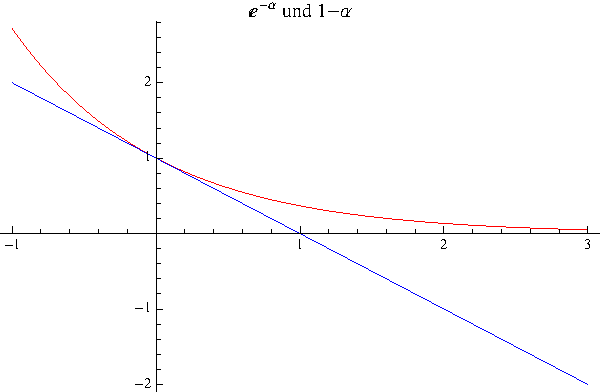
\includegraphics[width=1\columnwidth]{figs/borelcantelli}
\par\end{centering}

\caption{Skizze zu Borel-Cantelli}


\end{figure}
 Also gilt
\begin{eqnarray*}
P\left(\bigcap_{m\geq n}A_{m}^{c}\right) & = & \lim_{k\to\infty}P\left(\bigcap_{m=n}^{n+k}A_{m}^{c}\right)\\
 & \leq & \lim_{k\to\infty}\prod_{m=n}^{n+k}\exp\left(-P\left(A_{m}\right)\right)\\
 & = & \lim_{k\to\infty}\exp\left(-\sum_{m=n}^{n+k}P\left(A_{m}\right)\right)\\
 & = & 0
\end{eqnarray*}
da $\sum P\left(A_{m}\right)=+\infty$
\end{proof}

\section{Unabhängige Zufallsvariablen}


\paragraph*{Ziel:}

Wir hatten gezeigt:
\[
X_{i}\in\mathcal{L}^{2}
\]
unkorreliert mit 
\[
\sup_{i}\sigma^{2}\left(X_{i}\right)<\infty
\]
Dann gilt
\[
\lim_{n\to\infty}\frac{1}{n}\sum_{i=1}^{n}\left(X_{i}-\mathbb{E}\left[X_{i}\right]\right)=0\ P-f.s.
\]
Wir zeigen nun: $X_{i}\in\mathcal{L}^{1}$ unabhängig und identisch
verteilt (iid). Dann gilt
\[
\underset{\text{empirisches Mittel}}{\frac{1}{n}\sum_{i=1}^{n}X_{i}}\to\mathbb{E}\left[X_{1}\right]=:m
\]
Empirisches Mittel $\to$erwartetes Resultat eines einzelnen Versuches.
\begin{defn}
Eine Familie $\left(X_{i}\right)_{i\in I}$ von Zufallvariabeln auf
$\left(\Omega,\mathcal{A},\mathbb{P}\right)$ heißt unabhängig, falls
die von den Zufallsvariablen erzeugten Familie von $\sigma$-Algebren
\[
\left(\sigma\left(X_{i}\right)\right)_{i\in I}\ \left(\sigma\left(X_{i}\right)=\left\{ \left\{ x\in A|A\in\mathcal{B}\left(\overline{\mathbb{R}}\right)\right\} \right\} \right)
\]
unabhängig ist.\end{defn}
\begin{rem}
Sei $\left(X_{i}\right)_{i\in I}$ unabhängig
\[
h_{i}:\bar{\mathbb{R}}\to\bar{\mathbb{R}}\text{ meßbar}
\]
Dann gilt
\[
y_{i}=h_{i}\left(X_{i}\right)\ i\in I
\]
definiert eine Familie unabhängiger Zufallsvariablen.\end{rem}
\begin{proof}
Es gilt
\[
y_{i}^{-1}\left(A\right)=\underset{\in\sigma\left(X_{i}\right)}{\underbrace{X_{i}^{-1}\circ\underset{\in\mathcal{B}\left(\bar{\mathbb{R}}\right)}{\underbrace{h_{i}^{-1}\left(A\right)}}}}\ \mathcal{A}\in\mathcal{B}\left(\bar{\mathbb{R}}\right)
\]
D.h.
\[
\sigma\left(y_{i}\subseteq\sigma\left(X_{I}\right)\right)
\]
\end{proof}
\begin{prop}
Seien $X_{1},X_{2},\ldots\geq0$ unabhängig. Dann 
\[
\mathbb{E}\left[X_{1}\ldots X_{n}\right]=\prod_{i=1}^{n}\mathbb{E}\left[X_{i}\right]
\]
\end{prop}
\begin{proof}
OBdA $n=2$ (Rest per Induktion). Angenommen $\left(X_{1}=X,X_{2}=Y\right)$
\[
X=\sum\alpha_{j}+\1_{A_{j}},\ Y=\sum\beta_{j}\1_{B_{j}}
\]
mit $A_{i}$ von $B_{i}$ unabhängig. Dann gilt
\begin{eqnarray*}
\mathbb{E}\left[X\ Y\right] & = & \sum_{i,j}\alpha_{j}\beta_{i}\underset{{=P\left(A_{j}\cap B_{i}\right)\atop =P\left(A_{j}\right)\cdot P\left(B_{i}\right)}}{\underbrace{\mathbb{E}\left[\1_{A_{j}}\cdot\1_{B_{i}}\right]}}\\
 & = & \sum_{i,j}\alpha_{j}\beta_{i}P\left(A_{j}\right)\cdot P\left(B_{i}\right)\\
 & = & \mathbb{E}\left[X\right]\cdot\mathbb{E}\left[Y\right]
\end{eqnarray*}
Für allgemeine Zufallsvariablen, wähle 
\[
X_{n}:=\sum_{k=0}^{n\cdot2^{n}-1}k\cdot2^{-n}\1_{\left\{ k\cdot2^{-n}\leq X<\left(k+1\right)2^{-n}\right\} }
\]
analog für $Y_{n}$. Dann gilt
\[
X_{n}\nearrow X,\ Y_{n}\nearrow Y
\]
und $X_{n}$ und $Y_{n}$ sind unabhängig. Mit monotoner Konvergenz
folgt dann
\begin{eqnarray*}
\mathbb{E}\left[X\cdot Y\right] & = & \lim_{n\to\infty}\mathbb{E}\left[X_{n}\cdot Y_{n}\right]\\
 & = & \lim_{n\to\infty}\left(\mathbb{E}\left[X_{n}\right]\cdot\mathbb{E}\left[Y_{n}\right]\right)\\
 & \overset{\text{monotone}}{\underset{Konvergenz}{=}} & \mathbb{E}\left[X\right]\cdot\mathbb{E}\left[Y\right]
\end{eqnarray*}
\end{proof}
\begin{rem}
\textbf{(i)} Da $X,Y\in\mathcal{L}^{2}$
\[
\mathbb{E}\left[X\cdot Y\right]=\mathbb{E}\left[X\right]\mathbb{E}\left[Y\right]+2cov\left(X,Y\right)
\]
gilt Unabhängigkeit$\Rightarrow$Unkorreliert.\\
\textbf{(ii)} Die Umkehrung gilt i.d.R. nicht
\[
X\sim\mathcal{N}\left(0,1\right)\ y=x^{2}
\]
Dann gilt
\begin{eqnarray*}
\mathbb{E}\left[X\cdot Y\right] & = & \mathbb{E}\left[X^{3}\right]=0\\
 & = & \mathbb{E}\left[X\right]\mathbb{E}\left[X^{2}\right]
\end{eqnarray*}
Aber $X,Y$ nicht unabhängig!\end{rem}
\begin{cor}
Seien $X,Y\in\mathcal{L}^{1}$ unabhängig. Dann gilt
\[
X\cdot Y\in\mathcal{L}^{1}
\]
und $\mathbb{E}\left[X\cdot Y\right]=\mathbb{E}\left[X\right]\cdot\mathbb{E}\left[Y\right]$.
\end{cor}

\section{Kolmogorov'sches Gesetz der großen Zahlen}
\begin{prop}
(Kolmogorov)

Seien $\left(X_{i}\right)_{i\in\mathbb{N}}$ i.i.d. ZVen in $\mathcal{L}^{1}$
mit $m:=\mathbb{E}\left[X_{i}\right]$ $i\in\mathbb{N}$. Dann gilt
\begin{equation}
\frac{1}{n}\sum_{i=1}^{n}X_{i}\to m\ P-f.s.\label{eq:kolmogorov}
\end{equation}

\end{prop}

\begin{prop}
(Etenadi)

Seien $\left(X_{i}\right)_{i\in\mathbb{N}}$ \emph{paarweise }unabhängig
in $\mathcal{L}^{1}$, identisch verteilt. Dann gilt \ref{eq:kolmogorov}
\[
\frac{1}{n}\sum_{i=1}^{n}X_{i}\to m\ P-f.s.
\]
\end{prop}
\begin{proof}
(Etanadi)

Es seien oBdA $X_{i}\geq0$ (sonst auf $X_{i}^{+}$ und $X_{i}^{-}$
getrennt anwenden).
\begin{description}
\item [{(A)}] Wir zeigen zunächst: wir können die $X_{i}$ abschneiden.
Sei dazu 
\begin{eqnarray*}
\tilde{X}_{i} & = & \1_{\left\{ X_{i}<1\right\} }X_{i}\\
 & (= & h_{i}\left(X_{i}\right),h\left(x\right)=x\cdot\1_{\left\{ X<i\right\} }
\end{eqnarray*}
D.h. die $\tilde{X}_{i}$ sind paarweise unabhängig. Sei $\tilde{S}_{n}:=\sum_{i=1}^{n}\tilde{X}_{i}$.
Wir wollen zeigen:
\begin{equation}
P\left[\lim_{n\to\infty}\frac{1}{n}\left(S_{n}-\tilde{S}_{n}\right)=0\right]=1\label{eq:etanadi}
\end{equation}
Wir wenden dazu Borell-Cantelli an. Es gilt
\begin{eqnarray*}
\sum_{n\geq1}\mathbb{P}\left[X_{n}\neq\tilde{X}_{n}\right] & = & \sum_{n\geq1}P\left[X_{n}\geq n\right]\\
 & \overset{\text{gleichmäßig}}{\underset{\text{Verteilt}}{=}} & \sum_{n\geq1}P\left[X_{1}\geq n\right]\\
 & = & \sum_{n\geq1}\sum_{k=n}^{\infty}P\left[X_{1}\in[k,k+1)\right]\\
 & = & \sum_{k=1}^{\infty}\underset{\mathbb{E}\left[k\cdot\1_{\left\{ X_{1}\in[k,k+1)\right\} }\right]\leq\mathbb{E}\left[X_{1}\cdot\1_{\left\{ X\in[k,k+1)\right\} }\right]}{\underbrace{k\cdot P\left[X_{1}\in[k,k+1)\right]}}\\
 & \leq & \mathbb{E}\left[X_{1}\right]<\infty
\end{eqnarray*}
Mit Borel-Cantelli gilt dann
\[
P\left[X_{n}\neq\tilde{X}_{n}\text{ undendlich oft}\right]=0
\]
und somit gilt \ref{eq:etanadi}
\end{description}
\end{proof}
\printindex{}

\end{document}